\newpage
\section{Geometria de uma e duas câmeras}\label{sec.geo-1-2-cam}

\subsection{O espaço projetivo em duas dimensões}\label{sec.espaco-P2}

Para a compreensão mínima das técnicas mais importantes investigadas nessa dissertação, faz-se necessária a revisão condensada de um arcabouço notacional e conceitual que está disperso na literatura.

\subsubsection{A reta}\label{sec.reta}


Sabe-se que uma reta no plano $\mathbb{R}^{2}$ pode ser representada pela equação $a\,x+b\,y+c=0$, onde a reta fica perfeitamente determinada pelos valores das constantes $a,b,c$. Desta forma, podemos representar retas através de vetores, e assim a reta $a\,x+b\,y+c=0$ seria representada por $\lightrgb = (a,b,c)^\top \in \mathbb{R}^{3}$, utilizando o símbolo em negrito $\lightrgb$ para indicar tal vetor escrito em coluna, por padrão. Nota-se que a relação entre uma dada reta e o seu respectivo vetor não é biunívoca, pois o vetor $k\,(a,b,c)^\top$, tal que $k\neq 0$, representa a reta $k\,a\,x+k\,b\,y+k\,c=0$ que é a mesma reta $a\,x+b\,y+c=0$. Temos, então, infinitos vetores que representam uma mesma reta e formam uma {\it classe de equivalência}, onde essa classe pode ser representada por qualquer um de seus vetores. Os vetores de uma classe de equivalência, definida pela multiplicação por um escalar, são conhecidos como vetores {\it homogêneos}. O conjunto de classes de equivalência de vetores em $\mathbb{R}^{3} - (0,0,0)^\top$ forma o {\it Espaço Projetivo} $\mathbb{P}^{2}$. O vetor $(0,0,0)^\top$ foi excluído por não representar reta alguma. Após essas considerações, dizemos que uma reta no plano projetivo é representada pelo vetor $(a,b,c)^\top$ em {\it coordenadas homogêneas}.\\

\subsubsection{O ponto}\label{sec.ponto}


Sabemos que em $\mathbb{R}^{2}$ os pontos são representados através de pares ordenados do tipo $(x,y)$, e assim cada ponto pode ser identificado como um vetor $(x,y)^\top$. Os vetores em coordenadas homogêneas que se referem a pontos serão representados pelo símbolo em negrito $\x$, configurando uma terceira dimensão cuja coordenada é 1. Desse jeito, $\x=(x,y,1)^\top$. Sabemos também que um ponto $(x,y)$ pertence a uma reta $(a,b,c)^\top$ se, e somente se, $a\,x+b\,y+c=0$, ou, matricialmente:

\begin{equation*}
(x,y,1)^\top 
\begin{pmatrix}
 a  \\ 
 b  \\ 
 c 
 \end{pmatrix} 
 = 0 \qquad 
 \text{ou} 
 \qquad \x ^\top\lightrgb = 0.
\end{equation*}

Ou seja, temos um ponto de $\mathbb{R}^{2}$ representado como um vetor com três coordenadas. Observe que para $k\neq 0$, temos:

\begin{equation*}
(k\,x,k\,y,k)^\top 
\begin{pmatrix}
 a  \\ 
 b  \\ 
 c 
 \end{pmatrix} 
 = 0
 \qquad \Leftrightarrow \qquad
 (x,y,1)^\top
\begin{pmatrix}
 a  \\ 
 b  \\ 
 c 
 \end{pmatrix} 
 = 0.
\end{equation*}

Portanto,  variando $k$, podemos considerar os vetores em coordenadas homogêneas $(k\,x,k\,y,k)^\top \in \mathbb{P}^2$, como representantes do mesmo ponto $(x,y) \in \mathbb{R}^2$, e podemos resgatar nossa representação original aplicando o procedimento $(x/k,y/k)^\top$, pois $k \ne 0$.

\begin{figure}[!htb]
\centering
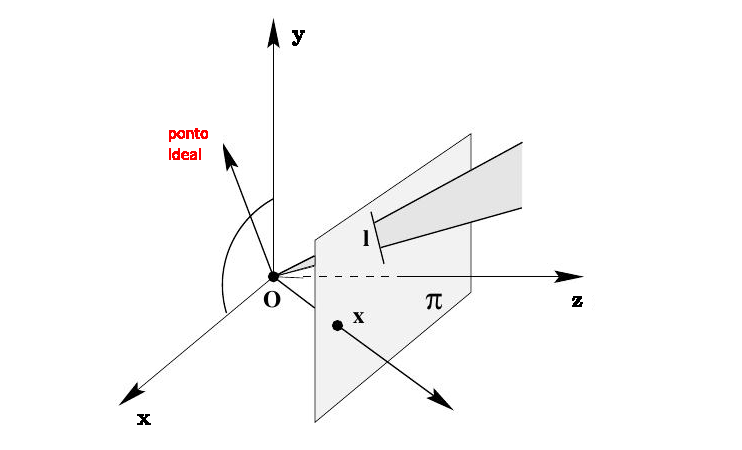
\includegraphics[scale=1]{espaco_P2}
\caption{\textit{O plano $\bpi$ representa o espaço projetivo $\mathbb{P}^2$. Pontos e retas pertencentes a esse espaço são representados, respectivamente, por vetores e planos que passam pela origem do $\mathbb{R}^3$. O ponto ideal é representado por um vetor que pertence ao plano $x\,y$, o qual é paralelo ao plano $\bpi$. O plano $x\,y$ representa a reta no infinito.}}
\label{plano_P2}
\end{figure}

Geometricamente, podemos pensar no plano projetivo como um conjunto de retas passando pela origem do $\mathbb{R}^3$, onde cada reta representa um único ponto, que é a interseção dessa reta com o plano $\mathbb{P}^2$. Analogamente, retas em $\mathbb{P}^2$ são formadas pela interseção de $\mathbb{P}^2$ com planos em $\mathbb{R}^3$. Na figura \ref{plano_P2}, observamos como a interseção da reta com o plano define um ponto, assim como a interseção de dois planos definem uma reta, com a vantagem de se incluir na representação o ponto ideal $(x,y,0)^\top$ e a reta no infinito que serão definidos mais adiante.


Como a representação de um ponto ou uma reta por vetores em coordenadas homogêneas não é alterada pela multiplicação por um escalar,  para determinarmos um ponto ou uma reta precisamos apenas de duas componentes do vetor, pois a terceira componente pode ser configurada como escala. Assim, dizemos que um ponto ou uma reta tem dois graus de liberdade.
\\

\subsubsection*{Retas determinadas por dois pontos e a interseção de duas retas}

A representação de retas em coordenadas homogêneas nos permite calcular a interseção de duas retas usando o produto vetorial. Sabemos que o produto vetorial de dois vetores, digamos $\lightrgb\times\lightrgb'$ em $R^3$ resulta num terceiro vetor que é ortogonal ao plano definido pelos vetores $\lightrgb$ e $\lightrgb'$. Em particular, esse terceiro vetor $\lightrgb\times\lightrgb'$ será ortogonal a qualquer dos vetores $\lightrgb$ e $\lightrgb'$, assim seu produto escalar é zero

\begin{equation*}
\lightrgb\cdot(\lightrgb\times\lightrgb')=\lightrgb'\cdot(\lightrgb\times\lightrgb')=0.
\end{equation*}
O produto escalar também pode ser representado por multiplicação matricial,

\begin{equation}\label{eq.pro-vet}
\lightrgb^\top(\lightrgb\times\lightrgb')=\lightrgb'^\top(\lightrgb\times\lightrgb')=0,
\end{equation}
e sendo $\x$ o ponto de interseção entre as duas retas temos

\begin{equation}\label{eq.pro-vet-2}
\lightrgb^\top\x=\lightrgb'^\top\x=0
\end{equation}
onde, comparando \ref{eq.pro-vet} e \ref{eq.pro-vet-2},

\begin{equation*}
\x=\lightrgb\times\lightrgb'.
\end{equation*}


Com argumento análogo podemos constatar que dois pontos definem uma reta através do produto vetorial entre eles, pois basta verificar que dois pontos $\x$ e $\x'$ pertencem a reta definida por

\begin{equation*}
\lightrgb=\x\times\x'.
\end{equation*}\\


\noindent {\bf Pontos ideais e a reta no infinito.}

Duas retas paralelas no espaço Euclidiano têm equações

\begin{equation*}
a\,x+b\,y+c=0\qquad\text{e}\qquad a\,x+b\,y+c'=0
\end{equation*}
com coordenadas homogêneas

\begin{equation*}
\lightrgb=(a,b,c)^\top\qquad\text{e}\qquad\lightrgb'=(a,b,c')^\top.
\end{equation*}
Computando a interseção entre as duas retas e ignorando o fator de escala $(c'-c)$ temos

\begin{equation*}
\begin{array}{rcl}
\lightrgb\times\lightrgb'&=&(a,b,c)^\top\times(a,b,c')^\top\\
&=&(c'-c)\,(b,-a,0)^\top\\
&=&(b,-a,0)^\top,
\end{array}
\end{equation*}
e se tentarmos encontrar as coordenadas não homogêneas do ponto de interseção temos

\begin{equation*}
\left(\frac{b}{0},\frac{-a}{0}\right)^\top,
\end{equation*}
o que não faz sentido matematicamente mas sugere que o ponto tem coordenadas que tendem ao infinito. Vetores homogêneos $(x,y,z)^\top$ com $z\neq0$ correspondem a pontos finitos em $R^2$ e, se $z=0$, os pontos são conhecidos como \textit{pontos ideais} ou \textit{pontos no infinito} no plano projetivo.

Se tomarmos um ponto no infinito genericamente $\x=(x,y,0)^\top$ percebemos que ele pertence a uma determinada reta $\lightrgb_\infty=(0,0,1)^\top$, pois

\begin{equation*}
\lightrgb_\infty^\top \x=(0,0,1)
\begin{pmatrix}
x\\
y\\
0
\end{pmatrix}
=0,
\end{equation*} 
e tal reta é conhecida como \textit{reta no infinto}. Assim, no plano projetivo temos que retas paralelas se encontram em ponto no infinito e o conjunto de pontos no infinito constituem a reta no infinito.

Um fato interessante sobre pontos no infinito é que eles são as direções das retas no plano projetivo $\mathbb{P}^2$. Um feixe de retas paralelas, que se intersectam num mesmo ponto no infinito, têm a mesma direção. Observa-se que a interseção de uma reta qualquer $\lightrgb=(a,b,c)^\top$ com a reta no infinito $\lightrgb_\infty=(0,0,1)^\top$,

\begin{equation*}
\lightrgb\times \lightrgb_\infty=(b,-a,0),
\end{equation*}
é um vetor que, em coordenadas não homogêneas $(b,-a)$, é ortogonal ao vetor $(a,b)$, que é o vetor normal à reta dada $\lightrgb=(a,b,c)^\top$. Assim $(b,-a)$ constitui-se a direção da reta $\lightrgb$, e como a reta no infinito contém todos os pontos do tipo $(b,-a,0)$, dizemos que a reta no infinito é o conjunto de direções das retas no plano projetivo $\mathbb{P}^2$.\\

\subsubsection{A cônica}\label{sec.definicao-conica}


Em Geometria Euclidiana, as cônicas são de três tipos principais: elipse, hipérbole e parábola. São definidas, algebricamente, por uma equação do segundo grau em duas variáveis, considerando coordenadas não homogêneas:

\begin{equation*}
a\,x^2+b\,x\,y+c\,y^2+d\,x+e\,y+f=0.
\end{equation*}
Sabemos que um ponto pertence à cônica se ele é solução da equação acima, a qual pode ser representada utilizando multiplicação matricial e vetores em coordenadas homogêneas,
\begin{equation*}
(x,y,1) 
 \begin{bmatrix}
a & b/2 & d/2\\
b/2 & c & e/2\\
d/2 & e/2 & f
\end{bmatrix}
 \begin{pmatrix}
x\\
y\\
1
\end{pmatrix}
 = 0.
\end{equation*}

Podemos generalizar essas coordenadas homogêneas multiplicando-se por um fator $x_3$ e definindo $x_1=x_3\,x$ e $x_2=x_3\,y$, e a equação fica
\begin{equation*}
a\,x_1^2+b\,x_1\,x_2+c\,x_2^2+d\,x_1\,x_3+e\,x_2\,x_3+f\,x_3^2=0.
\end{equation*}
Novamente, em notação matricial:

\begin{equation*}
(x_1,x_2,x_3) 
 \begin{bmatrix}
  a & b/2 & d/2\\
  b/2 & c & e/2\\
  d/2 & e/2 & f
  \end{bmatrix}
 \begin{pmatrix}
  x_1\\
  x_2\\
  x_3
  \end{pmatrix}
 = 0
 \qquad \text{ou} \qquad
 \x^\top C\,\x = 0.
\end{equation*}

Já que um ponto pertence à cônica se, e somente se, satisfaz a última equação, temos que $C$ fica definida como a matriz homogênea que representa uma cônica no plano projetivo $\mathbb{P}^2$,

\begin{equation*}
C =  \begin{bmatrix}
      a & b/2 & d/2\\
      b/2 & c & e/2\\
      d/2 & e/2 & f
      \end{bmatrix}.
\end{equation*}

Percebemos que as cônicas são representadas por matrizes $3\times3$ simétricas e, portanto, possuem seis variáveis. Usando uma dessas variáveis para fixar a escala, temos que as cônicas possuem cinco graus de liberdade, pois podemos por exemplo, dividir todas as coordenadas da matriz $C$ por $f$. Portanto, são necessários cinco pontos para que a mesma fique determinada.  \\

\subsubsection*{Retas tangentes a cônicas} 

Um conceito utilizado mais à frente nas investigações da calibração e estimação da pose relativa de câmeras é o de cônicas e seu envelope de retas tangentes. Uma reta tangente a uma cônica num ponto $\x$ qualquer tem a simples forma

\begin{equation*}
\lightrgb=C\x.
\end{equation*}
De fato, se a reta $\lightrgb$ passa por um ponto $\x$ temos que $\x^\top\lightrgb=0$, e se esse ponto $\x$ pertence à cônica $C$ então $\x^\top C\,\x=0$. Se $\x$ é o único ponto de interseção da reta com a cônica, comparando as duas relações  temos que $\lightrgb=C\x$ é a tangente procurada. Agora veremos que se a reta passa por mais um ponto na cônica, então toda a reta pertence à cônica e não é uma tangente.
Se a reta passa também por um outro ponto $\y$ na cônica, temos que $\y^\top C\,\y=0$ e $\lightrgb^\top\y=0$. Mas como $\lightrgb=C\x$ e considerando que $C$ é simétrica, temos

\begin{equation*}
\lightrgb^\top\y=(C\x)^\top\y=\x^\top C\,\y=0.
\end{equation*}  
Agora considerando todos os pontos em $\lightrgb=(\x+\alpha\y)$ parametrizados por $\alpha$, vamos verificar que todos eles pertencem à cônica $C$ usando as relações anteriores:

\begin{equation*}
(\x+\alpha\y)^\top C\,(\x+\alpha\y)=\x^\top C\,\x+\alpha\y^\top C\,\x+\x^\top C\,\alpha\y+\alpha\y^\top C\,\alpha\y=0,
\end{equation*}
já que cada uma das parcelas é zero. Assim toda a reta $\lightrgb$ ligando $\x$ e $\y$ está em $C$, que neste caso é dita ser uma cônica degenerada.\\

\subsubsection{Cônica dual ou reta}\label{sec.conica-dual} 

A cônica definida por $\x^\top C\,\x=0$ é chamada cônica de pontos já que é definida por uma equação que envolve pontos. Mas como pontos e retas têm a mesma representação por vetores de três componentes no plano projetivo $\mathbb{P}^2$, podemos também definir uma cônica por retas, chamada cônica dual ou de retas denotada por $C^*$, onde $\lightrgb^\top C^*\,\lightrgb=0$. Tal notação indica que $C^*$ é a matriz adjunta de $C$ e, sendo $C$ simétrica e não singular, $C^*=C^{-1}$. Com efeito, sendo $\lightrgb$ tangente à cônica $C$ temos $\lightrgb=C\,\x$, e sendo $C$ não singular temos que o ponto de tangência é $\x=C^{-1}\lightrgb$. Como $\x\in C$ temos que $\x^\top C\,\x=0$, assim

\begin{equation*}
\begin{array}{rcl}
\x^\top C\,\x&=&(C^{-1}\lightrgb)^\top C\,(
C^{-1}\lightrgb)\\
&=&\lightrgb^\top C^{-\top}\lightrgb\\
&=&\lightrgb^\top C^{-1}\lightrgb\\
&=&0.
\end{array}
\end{equation*}
Lembrando que $C^{-\top}=C^{-1}$ pois $C$ é simétrica. A relação $\lightrgb^\top C^*\,\lightrgb=0$ indica que as retas $\lightrgb_i$ são tangentes à cônica $C$, e por isso $C^*$ é conhecida como cônica envelope, como podemos visualizar na figura \ref{fig.conica-envelope}.

\begin{figure}[!htb]
\centering
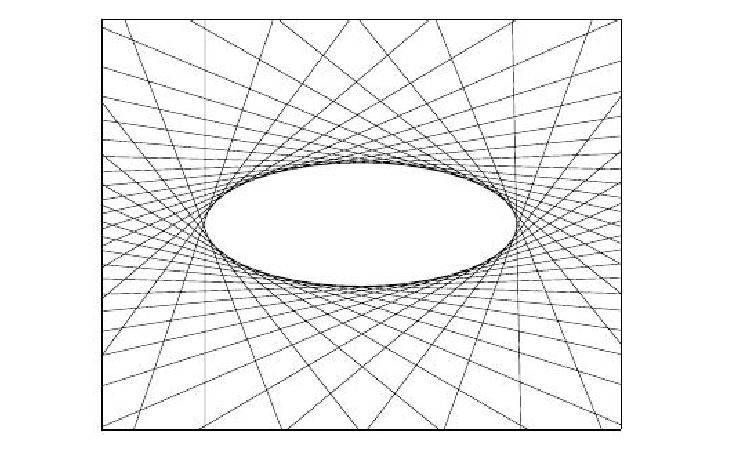
\includegraphics[scale=1]{conica-envelope}
\caption{\textit{A cônica $C$ é o envelope de todas as retas $\lightrgb_i$ que satisfazem $\lightrgb^\top C^*\,\lightrgb=0$.}}
\label{fig.conica-envelope}
\end{figure}

\subsubsection{Cônicas degeneradas}\label{sec.conicas-degeneradas}

Quando a matriz que representa a cônica não tem posto completo ocorrem cônicas degeneradas, daí a cônica será duas retas caso a matriz tenha posto $2$ ou uma reta repetida caso a matriz tenha posto $1$. A seguir dois exemplos de cônicas degeneradas, uma cônica ponto e uma cônica dual. A cônica 

\begin{equation*}
C=\lightrgb\,{\bf m}^\top+{\bf m}\,\lightrgb^\top
\end{equation*}
é uma cônica ponto composta por duas retas $\lightrgb$ e ${\bf m}$. Assim, se um ponto $\x\in\lightrgb$ então $\lightrgb^\top\x=0$ e esse ponto deve satisfazer $\x^\top C\,\x=0$. De fato,

\begin{equation*}
\begin{array}{rcl}
\x^\top C\,\x&=&\x^\top(\lightrgb\,{\bf m}^\top+{\bf m}\,\lightrgb^\top)\,\x\\
&=&\x^\top\lightrgb\,{\bf m}^\top\x+\x^\top {\bf m}\,\lightrgb^\top\x\\
&=&0\,{\bf m}^\top\x+\x^\top{\bf m}\,0\\
&=&0.
\end{array}
\end{equation*}
A argumentação é analoga caso $\x\in{\bf m}$. A equação de uma cônica dual degenerada é composta por pontos e a matriz correspondente tem posto 2 caso seja composta por dois pontos, ou posto 1 caso seja composta por um ponto repetido, 

\begin{equation*}
C^*=\x\,\y^\top+\y\,\x^\top.
\end{equation*}
De forma análoga à argumentação anterior podemos demosntrar que $C^*$ define um equação em retas,

\begin{equation*}
\lightrgb^\top\,C^*\lightrgb=0.
\end{equation*}

\subsubsection{A relação polo-polar}\label{sec.polo-polar}

Vimos anteriormente que uma reta $\lightrgb$ é tangente a uma cônica num ponto $\x$ se 

\begin{equation*}
\lightrgb=C\,\x.
\end{equation*}
Mas se o ponto $\x$ não pertence à cônica $C$ então temos uma relação denominada \textit{polo-polar}, onde a reta $\lightrgb$ é chamada reta \textit{polar} de $\x$, e $\x$ é chamado o \textit{polo} da reta $\lightrgb$, conforme a ilustração na figura \ref{fig.polo-polar}.

A reta polar $\lightrgb=C\,\x$ intercepta a cônica 
$C$ em dois pontos $\y_1$ e $\y_2$, e as retas tangentes à cônica $C$ nesses dois pontos se interceptam em $\x$. De fato, considere o ponto $\y_1 \in C$ e a reta tangente a esse ponto ${\bf m}=C\,\y_1$. Essa tangente contém o ponto $\x$ se 

\begin{equation*}
\x^\top{\bf m}=0\qquad\text{ou}\qquad\x^\top C\,\y_1=0,
\end{equation*}  
e, usando a simetria da cônica $C$ e aplicando a transposição em $\x^\top C$, temos

\begin{equation*}
\x^\top C\,\y_1=(C\,\x)^\top\y_1=0,
\end{equation*}
mostando que o ponto $\y_1$ pertence à reta $\lightrgb=C\,\x$. Assim, a reta $\lightrgb$ intercepta a cônica $C$ no ponto $\y_1$, no qual a tangente a $C$ contém o ponto $\x$. Observa-se que se o ponto $\x$ se aproxima da cônica $C$, os dois pontos $\y_1$ e $\y_2$ vão se aproximando um do outro, e quando ponto $\x$ pertence à conica $C$ a reta polar se torna a reta tangente. O argumento é análogo para $\y_2$.\\


\begin{figure}[!htb]
\centering
\subfloat[]{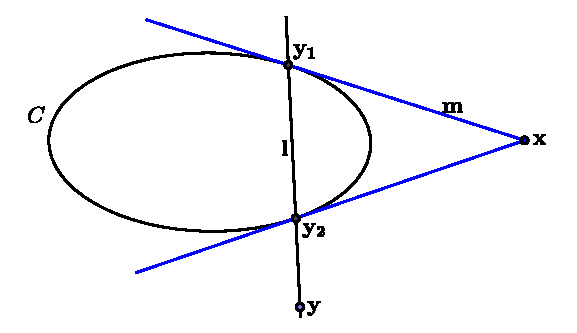
\includegraphics[scale=.81]{polo-polar}}
\quad
\subfloat[]{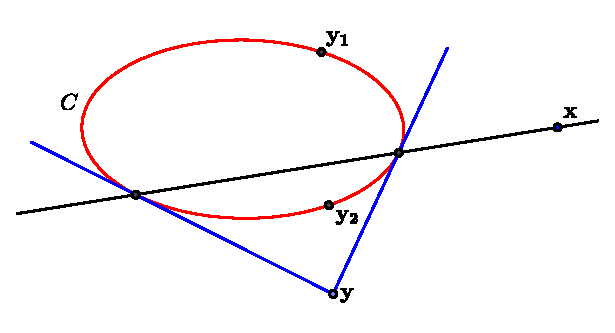
\includegraphics[scale=.81]{polo-polar-simetria}}
\caption{\textit{(a) A reta $\lightrgb=C\,\x$ é a reta polar de $\x$, e o ponto $\x=C^{-1}\lightrgb$ é o polo da reta $\lightrgb$. Os pontos $\x$ e $\y$ são chamados conjugados, pois obedecem à relação $\y^\top C\,\x=0$. (b) Duplicação da figura para visualização da simetria da relação polo-polar. O ponto $\x$ pertence à reta polar de $\y$.}}
\label{fig.polo-polar}
\end{figure}






\noindent {\bf Pontos conjugados.}

Quando um ponto $\y$ qualquer pertence à reta polar $\lightrgb=C\,\x$ temos que 

\begin{equation*}
\y^\top\lightrgb=\y^\top C\,\x=0,
\end{equation*}
e quaisquer dois pontos que satisfazem a relação $\y^\top C\,\x=0$ são chamados \textit{conjugados} com relação à cônica $C$. Repare que o ponto $y$ não precisa necessariamente pertencer à cônica. Mais anida, se um ponto $\y$ está na reta polar de $\x$, então $\x$ está na reta polar de $\y$. Como vimos, se $\y$ está na reta polar de $\x$ vale a relação $\y^\top C\,\x=0$, e tomando a transposta temos que $\x^\top C\,\y=0$, pois $C$ é simétrica. 
%Existe uma relacao de conjugacao para retas, digamos ${\bf l}$ e ${\bf m}$: ${\bf l}^\top C^*{\bf m}=0$.


\subsubsection{Transformações projetivas em $\mathbb{P}^2$}\label{sec.trans-proj-H}

A tranformação projetiva também conhecida como projetividade, colineação ou homografia,  é uma função (invertível) que transforma pontos no plano $\mathbb{P}^2$ para pontos no plano $\mathbb{P}^2$ preservando a colinearidade desses pontos. Mais formalmente, uma função $h:\mathbb{P}^2\rightarrow\mathbb{P}^2$ é uma transformação projetiva se, e somente se, existe uma matriz $H_{3\times3}$ onde para cada ponto $\x\in\mathbb{P}^2$ temos que $h(\x)=H\,\x$. De fato, dados três pontos $\x_1$, $\x_2$ e $\x_3$ na mesma reta $\lightrgb$, temos que $\lightrgb^\top\x_i=0$ para $i=1,2 \,\,\,\text{e}\,\,\, 3$. Seja dada ainda uma matriz invertível $H_{3\times3}$. Definindo
\begin{equation*}
\lightrgb'=H^{-\top}\lightrgb \qquad\text{e}\qquad \x'_i=H\,\x_i,
\end{equation*}
vemos que todos os pontos $\x'_i$ pertencem à reta $\lightrgb'$, pois

\begin{equation*}
\begin{array}{rcl}
\lightrgb'^\top\x'_i&=&(H^{-\top}\lightrgb)^\top H\,\x_i\\
&=&\lightrgb^\top H^{-1}H\,\x_i\\
&=&\lightrgb^\top\x_i=0
\end{array}
\end{equation*}
preservando assim, a colinearidade dos pontos. A implicação direta é demasiadamente grande. A argumentação mostra que qualquer transformação linear aplicada a coordenadas homogêneas é uma transformação projetiva em $\mathbb{P}^2$, ou seja, a transformação projetiva é simplesmente uma transformação linear em $\mathbb{R}^3$. Podemos ver que o efeito da matriz $H$ não é alterado pela multiplicação por um escalar diferente de zero na equação

\begin{equation*}
\x'=H\,\x,
\end{equation*}
pois os pontos permanecem colineares após a transformação, alterando apenas a escala. Assim, a matriz $H$ é homogênea, e apenas a razão entre os seus elementos é significante, ou seja, são nove elementos mas oito graus de liberdade. Os pontos $\x\leftrightarrow\x'$ são chamados {\it pontos correspondentes}.\\

\noindent {\bf Transformação de retas.}

Na argumentação anterior vimos que a reta $\lightrgb'$ foi definida na forma $\lightrgb'=H^{-\top}\lightrgb$. Tal definição não foi em vão, pois a definição nesta forma garante que os pontos depois de transformados permaneçam colineares. Assim, a transformação projetiva de pontos nos dá essa regra para transformação projetiva de retas.\\

\noindent {\bf Transformação de cônicas.}

Invertendo a função $\x'=H\,\x$ temos que $\x=H^{-1}\x'$, e substituindo $\x$ na equação matricial de uma cônica $\x^\top C\,\x=0$ temos

\begin{equation*}
\begin{array}{rcl}
\x^\top C\,\x&=&(H^{-1}\x')^\top C\,H^{-1}\x'\\
&=&\x'^\top H^{-\top}C\,H^{-1}\x'\\
&=&\x'^\top C'\x'=0
\end{array}
\end{equation*}
onde $\x'^\top C'\x'=0$ é a equação matricial da cônica depois de aplicada a transformação projetiva, com $C'=H^{-\top}C\,H^{-1}$ sendo a regra para a transformação de cônicas.


\subsubsection{A geometria projetiva de uma dimensão}\label{sec.geometria-1D}
Vamos abrir um parênteses na discussão sobre o plano ${\mathbb{P}^2}$ para discorrer brevemente sobre a {\it reta projetiva} ${\mathbb{P}}$. A reta projetiva tem muita similaridade com o plano projetivo, pois pontos na reta são representados em coordenadas homogêneas (vetores com duas componentes) e são projetivamente transformados de acordo com uma homografia $H_{2\times2}$. Na reta projetiva ${\mathbb{P}}$ os pontos têm as seguintes notação e transformação projetiva: 

\begin{equation}\label{eq.ponto-homografia-em-P}
\overline{\x}=
\begin{pmatrix}
x_1\\
x_2
\end{pmatrix}
\qquad\text{e}\qquad
\overline{\x}'=H\,\overline{\x}.
\end{equation}
Pontos no infinito têm a componente $x_2=0$.

\begin{figure}[!htb]
\centering
\subfloat[]{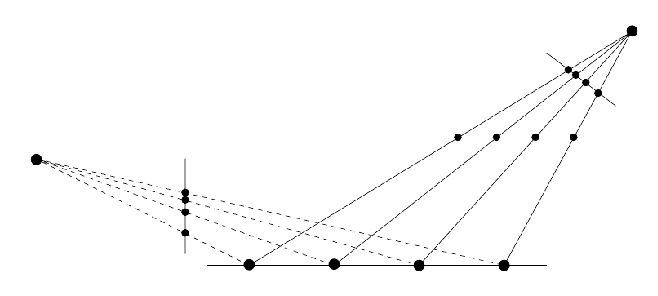
\includegraphics[scale=.9]{geometria-P1}}
\quad
\subfloat[]{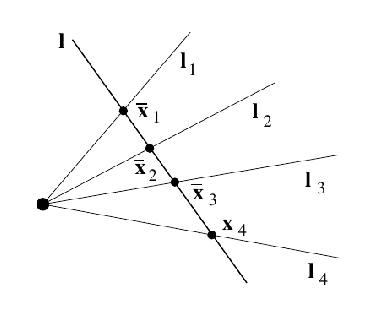
\includegraphics[scale=.9]{razao-cruzada-retas}}
\caption{$({\tt a})\,$\textit{Cada grupo de quatro pontos está relacionado aos outros grupos por uma transformação projetiva em ${\mathbb{P}}$. Como a razão cruzada é uma invariante, tais grupos possuem a mesma razão cruzada.}$\,({\tt b})\,$\textit{A razão cruzada das quatro retas é uma invariante projetiva do plano que as contém (ver subseção \ref{sec.hierarquia-transformacoes}). As retas contendo os quatro pontos podem ser vistas em ${\mathbb{P}^2}$ como planos de imagens, objetos planares, relacionados por centros de projeção.}}
\label{fig.razao-cruzada}
\end{figure}

\subsubsection*{A razão cruzada.}
A definição a seguir é uma \textit{invariante} (ver subseção \ref{sec.hierarquia-transformacoes}) básica da geometria projetiva. Dados quatro pontos numa reta, conforme a figura \ref{fig.razao-cruzada}, a razão cruzada é definida por 

\begin{equation*}
\text{cross}(\overline{\x}_1,\overline{\x}_2,\overline{\x}_3,\overline{\x}_4)=\frac{|\overline{\x}_1\,\overline{\x}_2||\overline{\x}_3\,\overline{\x}_4|}{|\overline{\x}_1\,\overline{\x}_3||\overline{\x}_2\,\overline{\x}_4|},
\end{equation*}
onde 

\begin{equation*}
|\overline{\x}_i\,\overline{\x}_j|=
\text{det}
\begin{bmatrix}
x_{i1}&x_{j1}\\
x_{i2}&x_{j2}
\end{bmatrix}.
\end{equation*}

Vamos verificar que a razão cruzada é uma invariante sob transformação projetiva, ou seja, dada uma homografia como a equação \ref{eq.ponto-homografia-em-P} temos que 

\begin{equation}\label{eq.invariante-cross}
\text{cross}(\overline{\x}'_1,\overline{\x}'_2,\overline{\x}'_3,\overline{\x}'_4)=\text{cross}(\overline{\x}_1,\overline{\x}_2,\overline{\x}_3,\overline{\x}_4).
\end{equation}
De fato,

\begin{equation*}
\begin{array}{rcll}
\text{cross}(\overline{\x}'_1,\overline{\x}'_2,\overline{\x}'_3,\overline{\x}'_4)&=&\displaystyle\frac{|\overline{\x}'_1\,\overline{\x}'_2||\overline{\x}'_3\,\overline{\x}'_4|}{|\overline{\x}'_1\,\overline{\x}'_3||\overline{\x}'_2\,\overline{\x}'_4|}&\text{como}\qquad\overline{\x}'=H\,\overline{\x}\\\\
&=&
\displaystyle\frac{|H\,\overline{\x}_1\,H\,\overline{\x}_2||H\,\overline{\x}_3\,H\,\overline{\x}_4|}{|H\,\overline{\x}_1\,H\,\overline{\x}_3||H\,\overline{\x}_2\,H\,\overline{\x}_4|}&\\\\
&=&
\displaystyle\frac{|H\,[\overline{\x}_1\,\overline{\x}_2]||H\,[\overline{\x}_3\,\overline{\x}_4]|}{|H\,[\overline{\x}_1\,\overline{\x}_3]||H\,[\overline{\x}_2\,\overline{\x}_4|]}&[\overline{\x}_i\,\overline{\x}_j]\quad\text{é matriz}      \\\\
&=&
\displaystyle\frac{|H|\,|\overline{\x}_1\,\overline{\x}_2|\,|H|\,|\overline{\x}_3\,\overline{\x}_4|}{|H|\,|\overline{\x}_1\,\overline{\x}_3|\,|H|\,|\overline{\x}_2\,\overline{\x}_4|}&\\\\
&=&
\displaystyle\frac{|\overline{\x}_1\,\overline{\x}_2||\overline{\x}_3\,\overline{\x}_4|}{|\overline{\x}_1\,\overline{\x}_3||\overline{\x}_2\,\overline{\x}_4|}&\\\\
&=&
\text{cross}(\overline{\x}_1,\overline{\x}_2,\overline{\x}_3,\overline{\x}_4),
\end{array}
\end{equation*}
e portanto a equação \ref{eq.invariante-cross} segue.

Como corolário, segundo \cite{kneebone}, existe homografia $H$ onde $\overline{\x}'_i=H\,\overline{\x}_i$ se, e somente se, $\text{cross}(\overline{\x}_1,\overline{\x}_2,\overline{\x}_3,\overline{\x}_4)=\text{cross}(\overline{\x}'_1,\overline{\x}'_2,\overline{\x}'_3,\overline{\x}'_4)$. 

%Como a implicação direta já foi feita na argumentação anterior, vamos fazer a implicação contrária. Sabemos que a razão cruzada é invariante sob projetividade, portanto
%
%\begin{equation*}
%\text{cross}(\overline{\x}_1,\overline{\x}_2,\overline{\x}_3,\overline{\x}_4)=\text{cross}(H\,\overline{\x}_1,H\,\overline{\x}_2,H\,\overline{\x}_3,H\,\overline{\x}_4).
%\end{equation*}
%Como
%
%\begin{equation*}
%\text{cross}(\overline{\x}_1,\overline{\x}_2,\overline{\x}_3,\overline{\x}_4)=\text{cross}(\overline{\x}'_1,\overline{\x}'_2,\overline{\x}'_3,\overline{\x}'_4),
%\end{equation*}
%temos que
%
%\begin{equation*}
%\text{cross}(\overline{\x}'_1,\overline{\x}'_2,\overline{\x}'_3,\overline{\x}'_4)=\text{cross}(H\,\overline{\x}_1,H\,\overline{\x}_2,H\,\overline{\x}_3,H\,\overline{\x}_4).
%\end{equation*}
%Assim,
%
%\begin{equation*}
%\overline{\x}'=H\,\overline{\x}.
%\end{equation*}

\subsubsection*{Retas concorrentes.}
Vimos que pontos e retas têm representações similares em ${\mathbb{P}^2}$ usando vetores homogêneos com três componentes. Daí, fazendo as devidas alterações, todo teorema relacionado a pontos são válidos também para retas, e dizemos que existe a {\it dualidade} entre pontos e retas no plano ${\mathbb{P}^2}$. Analogamente,  
quatro retas concorrentes em um único ponto têm geometria em ${\mathbb{P}}$ dual com quatro pontos colineares, assim a razão cruzada entre essas retas também é uma invariante sob projetividade. Conforme a figura \ref{fig.razao-cruzada}, o valor da razão cruzada entre as quatro retas é dado pelos pontos de interseção de uma quinta reta transversal a essas quatro, ou seja

\begin{equation*}
\text{cross}(\lightrgb_1,\lightrgb_2,\lightrgb_3,\lightrgb_4)=\text{cross}(\overline{\x}_1,\overline{\x}_2,\overline{\x}_3,\overline{\x}_4).
\end{equation*}
Tal asserção é devida ao teorema de \textit{Pappus} conforme \citep{springer64}. 



\subsubsection{Subgrupo de transformações projetivas}\label{sec.hierarquia-transformacoes}

As transformações projetivas se dividem em subgrupos de transformações com características mais específicas. Esses subgrupos são as \textit{isometrias}, \textit{similaridades}, \textit{afinidades} e a própria \textit{transformação projetiva}. Cada subgrupo mantém \textit{invariante} algumas propriedades do objeto ao qual a transformação está sendo aplicada. Por exemplo, a distância entre dois pontos num quadrado se mantém a mesma após a aplicação de uma transformação isométrica (translação, rotação e possível reflexão), mas pode variar após a aplicação de uma transformação de similaridade, a qual pode gerar um quadrado maior ou menor que o original. Portanto, distância entre dois pontos é uma invariante sob isometria mas não é sob similaridade.

\subsubsection*{Transformação isométrica.}
É representada pela matriz

\begin{equation*}
\begin{bmatrix}
\epsilon\,cos\,\theta&-sen\,\theta&t_x\\
\epsilon\,sen\,\theta&cos\,\theta&t_y\\
0&0&1
\end{bmatrix},
\end{equation*}
onde $\epsilon=\pm1$. Se $\epsilon=1$ a isometria preserva a orientação e é chamada \textit{Transformação Euclidiana} (composição de translação e rotação). Se $\epsilon=-1$ a isometria reverte a orientação. A transformação Euclidiana é o tipo de isometria mais importante, denotada por $H_E$ e representada pela matriz em forma de blocos

\begin{equation*}
H_E=
\begin{bmatrix}
R&{\bf t}\\
{\bf 0}^\top&1
\end{bmatrix}.
\end{equation*}
Sendo $R_{2\times2}$ uma matriz de rotação, ${\bf t}$ um vetor com duas componentes e ${\bf 0}=(0,0)^\top$ um vetor nulo, essa transformação tem três graus de liberdade, um para o ângulo de rotação em $R$ e dois para o vetor de translação. Assim, são necessários no mínimo dois pontos correspondentes $\x_i\leftrightarrow\x'_i$ para determinarmos a matriz da transformação Euclidiana. As invariantes são distância entre dois pontos, ângulo entre duas retas e área. 

\subsubsection*{Tranformação de similaridade.}
A transformação de similaridade é denotada por $H_S$ e é representada pela matriz 

\begin{equation*}
H_S=
\begin{bmatrix}
s\,cos\,\theta&-s\,sen\,\theta&t_x\\
s\,sen\,\theta&s\,cos\,\theta&t_y\\
0&0&1
\end{bmatrix},
\end{equation*} 
que neste caso é a composição de uma transformação Euclidiana com uma escala (sem reflexão) $s$. A transformação de similaridade preserva a forma dos objetos e tem quatro graus de liberdade, com o escalar $s$ contando para um grau a mais que a transformação Euclidiana. A similaridade também pode ser determinada usando dois pontos correspondentes e tem a matriz em bloco

\begin{equation*}
H_S=
\begin{bmatrix}
s\,R&{\bf t}\\
\,{\bf 0}^\top&1
\end{bmatrix}.
\end{equation*}
Com a mudança na escala das figuras, a área e a distância entre dois pontos não é mais a mesma após a transformação, mas os ângulos entre as retas não mudam, e pontanto, ângulo é uma invariante sob similaridade. Em particular, retas paralelas permanecem paralelas. A razão entre as distâncias antes e após a transformação permanece a mesma por conta do cancelamento da escala, e analogamente, a razão entre as áreas também permanece a mesma por conta do cancelamento do quadrado da escala.

\subsubsection*{Transformação afim.}
A transformação afim, ou afinidade, é uma transformação linear seguida de uma translação, denotada por $H_A$ e representada pela matriz

\begin{figure}[!htb]
\centering
\subfloat[]{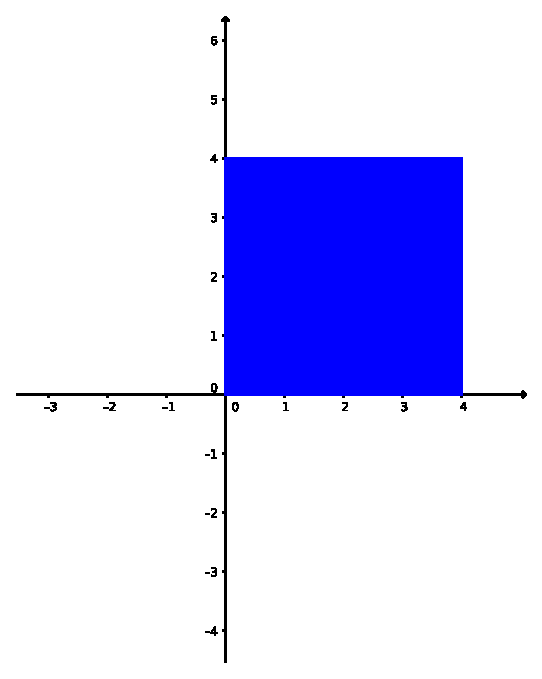
\includegraphics[scale=.35]{quadrado-1}}
\,
\subfloat[]{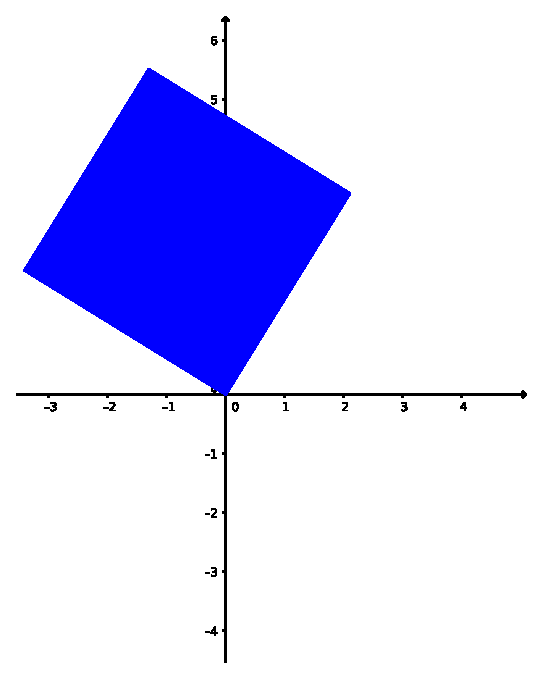
\includegraphics[scale=.35]{quadrado-2}}
\,
\subfloat[]{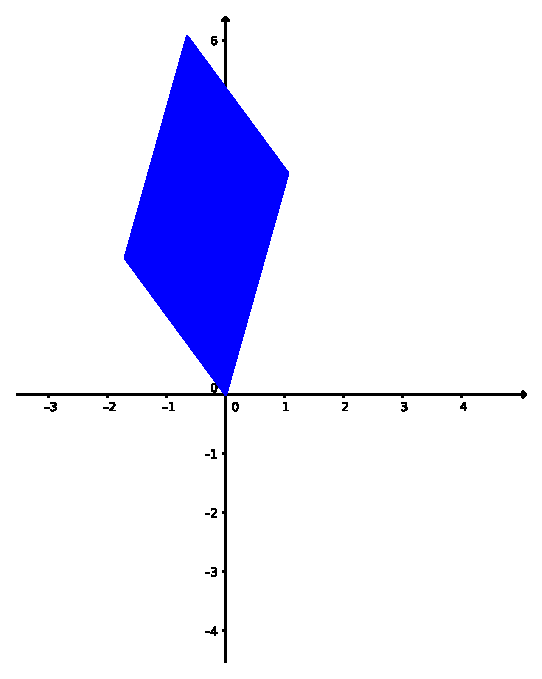
\includegraphics[scale=.35]{losango-1}}
\,
\subfloat[]{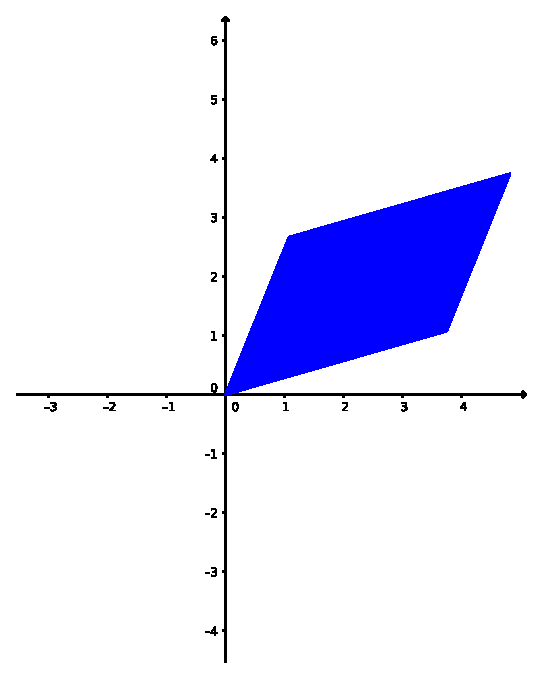
\includegraphics[scale=.35]{losango-2}}
\,
\subfloat[]{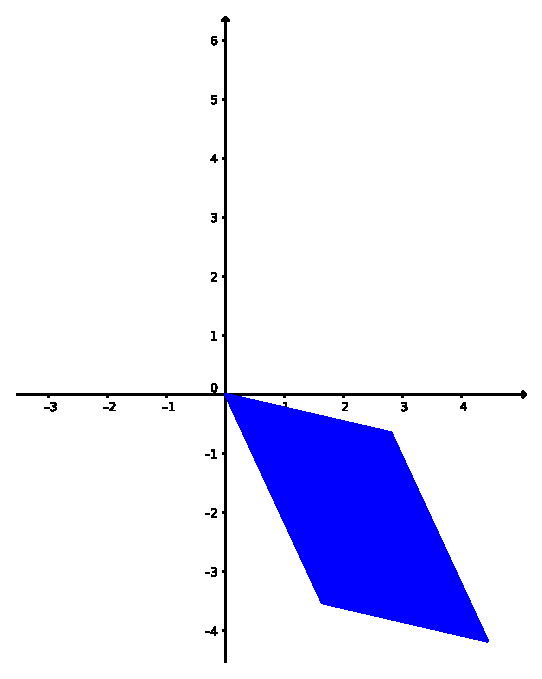
\includegraphics[scale=.35]{losango-3}}
\caption{$({\tt a})\,$\textit{Um quadrado.}$\,({\tt b})\,$\textit{Rotação $R(50^\circ)$.}$\,({\tt c})\,$\textit{Escala não uniforme $D$ com $\lambda_1=0,5$ e $\lambda_2=1,1$.}$\,({\tt d})\,$\textit{Rotação $R(-50^\circ)$.}$\,({\tt e})\,$\textit{Rotação final $R(-70^\circ)$.}}
\label{fig.angulos-afinidades}
\end{figure}

\begin{equation*}
H_A=
\begin{bmatrix}
a_{11}&a_{12}&t_x\\
a_{21}&a_{22}&t_y\\
0&0&1
\end{bmatrix}.
\end{equation*}
A matriz possui seis graus de liberdade correspondentes ao seis elementos da matriz, e são necessários três pontos correspondentes para determinarmos a matriz de afinidade que pode ser escrita em blocos como

\begin{equation*}
H_A=
\begin{bmatrix}
A&{\bf t}\\
{\bf 0}^\top&1
\end{bmatrix}.
\end{equation*}
Como uma forma de ajudar a entender os efeitos da matriz $A$ vamos decompô-la em transformações mais fundamentais

\begin{equation*}
A=R(\theta)R(-\phi)DR(\phi),
\end{equation*}
com uma matriz diagonal $D=diag(\lambda_1, \lambda_2)$ onde as componentes são escalares não-isotrópicos 
%\footnote{Isotrópico: É o que se diz de um corpo que, em todas as direções, apresenta as mesmas propriedades ópticas.} 
que alteram a escala nos eixos $x$ e $y$ respectivamente. Uma rotação $\phi$ que define o sentido de aplicação dos escalares da matriz $D$, uma rotação contrária $-\phi$ e uma última rotação $\theta$. Podemos visualizar os efeitos das rotações e dos escalares na figura \ref{fig.angulos-afinidades}. Os dois graus de liberdade a mais em relação a uma similaridade vêm do ângulo $\phi$ e da razão entre os escalares aplicados por $D$, $\frac{\lambda_1}{\lambda_2}$. 


Temos três importantes invariantes sob afinidade: retas paralelas se matêm paralelas, razão entre seguimentos de retas paralelas e razão entre as áreas. Mesmo que retas paralelas sejam invariantes, a afinidade não mantém, em geral, o ângulo entre retas nem a razão entre as distâncias correspondentes como acontece com a similaridade.

\subsubsection*{Transformações projetivas.}
É uma transformação linear mais geral de coordenadas homogêneas (já definida na subseção \ref{sec.trans-proj-H}), pois generaliza  a transformação de afinidade. Na forma de blocos temos a representação

\begin{equation*}
H_P=
\begin{bmatrix}
A&{\bf t}\\
{\bf v}^\top&v
\end{bmatrix},
\end{equation*}
onde ${\bf v}=(v_1,v_2)$. Como a matriz é $3\times3$ temos nove variáveis a serem determinadas, mas que se reduzem a oito tomando uma das variáveis para escala. Assim, precisamos de quatro pontos correspondentes para determinarmos os oito parâmetros da matriz. Além de manter a colinearidade dos pontos, uma invariante fundamental na transformação projetiva é a razão cruzada entre quatro pontos colineares, ou seja, a razão das razões de segmentos contidos numa mesma reta. Na figura \ref{fig.transformacoes-2D} podemos ver um resumo das características geométricas preservadas (em um quadrado, por exemplo) por cada subgrupo de transformação.   

\begin{figure}[!htb]
\centering
\subfloat{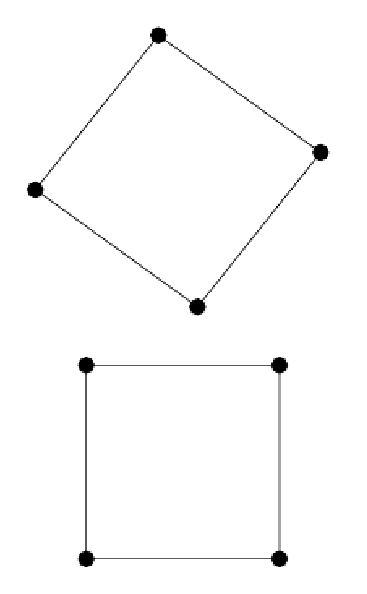
\includegraphics[scale=.6]{trans-euclidiana-2D}}
\qquad
\subfloat{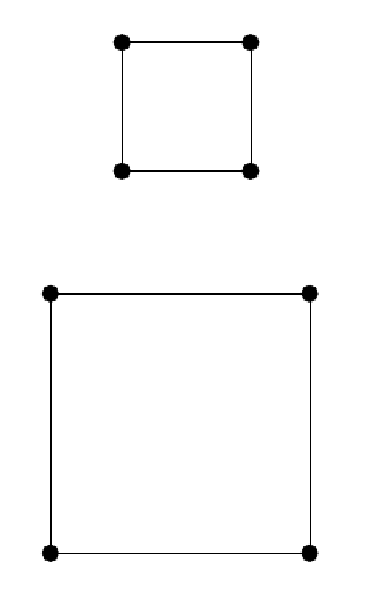
\includegraphics[scale=.6]{trans-similaridade-2D}}
\qquad
\subfloat{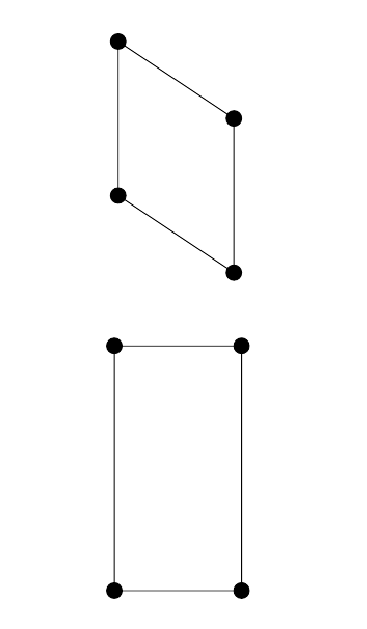
\includegraphics[scale=.6]{trans-afinidade-2D}}
\qquad
\subfloat{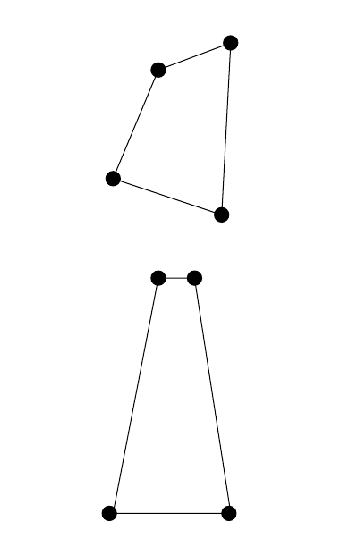
\includegraphics[scale=.6]{trans-projetividade-2D}}
\caption{\textit{Respectivamente, transformações: euclidiana, similaridade, afinidade, e projetividade.}}
\label{fig.transformacoes-2D}
\end{figure}

\subsection{O espaço projetivo em três dimensões}\label{sec.espaco-P3}


\subsubsection*{O ponto} 


Analogamente à representação de um ponto no plano $\mathbb{P}^2$, um ponto no espaço $\mathbb{P}^3$ é repesentado através de coordenadas homogêneas, acrescentando-se uma quarta coordenada ao vetor que representa esse ponto. Desta forma, $\X = (X_1,X_2,X_3,X_4)^\top$ e $X_4 \ne 0$, onde $\X$ é a representação em coordenadas homogêneas do ponto $(X,Y,Z)^\top \in \mathbb{R}^3$, e portanto um ponto nesse espaço tem três graus de liberdade. Para realizar tal mudança basta tomar 

\begin{equation*}
X=X_1/X_4 \,\, ,\, Y=X_2/X_4 \,\,\, \text{e} \,\,\, Z=X_3/X_4.
\end{equation*}

 

\subsubsection*{O plano}

Temos que a representação algébrica de um plano $\bpi$ no espaço $\mathbb{R}^3$ é dada pela equação
\begin{equation*}
\pi_1\,X+\pi_2\,Y+\pi_3\,Z+\pi_4=0,
\end{equation*}
onde $\pi_i$ são os coeficientes da equação. Um ponto em $\mathbb{R}^3$ pertence ao plano se, e somente se, satifaz a equação acima que na forma matricial usando a representação do ponto em coordenadas homogêneas fica

\begin{equation*}
  (\pi_1,\pi_2,\pi_3,\pi_4)^\top
 \begin{pmatrix}
  X\\
  Y\\
  Z\\
  1
  \end{pmatrix}
 = 0.
\end{equation*}
Fazendo as substituições 
\begin{equation*}
X=X_1/X_4 \,\, , \,\, Y=X_2/X_4 \,\,\,\, \text{e} \,\,\,\, Z=X_3/X_4 ,
\end{equation*}

generalizamos a representação do ponto e a equação se torna

\begin{equation*}
\begin{array}{ccc}
(\pi_1,\pi_2,\pi_3,\pi_4)^\top
  \begin{pmatrix}
  X_1\\
  X_2\\
  X_3\\
  X_4
  \end{pmatrix}
  = 0
& \qquad \text{ou} \qquad
& \bpi^\top \, \X = 0.
\end{array}
\end{equation*}

Desta forma, verificamos que, assim como os pontos, um plano $\bpi = (\pi_1,\pi_2,\pi_3,\pi_4)^\top$ fica inteiramente determinado por um vetor com quatro coordenadas em $\mathbb{P}^3$. Aqui temos uma analogia com o espaço $\mathbb{P}^2$, já que pontos e retas têm a mesma representação vetorial com três componentes naquele espaço, e a dualidade entre pontos e retas em $\mathbb{P}^2$ também se verifica entre pontos e planos em $\mathbb{P}^3$. Como multiplicar a equação algébrica de um plano por um escalar diferente de zero não altera o plano, temos que os planos possuem três graus de liberdade. Podemos dividir as três primeiras coordenadas pela última, por exemplo, e fixar uma escala.

Obs: As três primeiras coordenadas do vetor que representa o plano corresponde ao vetor normal ao plano, conforme definido em Álgebra Linear.
\\


\subsubsection*{A reta}

Uma reta pode ser definida passando por dois pontos. Em $\mathbb{P}^2$, como os dois pontos estão no mesmo plano, uma reta passando por esses dois pontos tem apenas dois graus de liberdade, conforme visto anteriormente. Mas em $\mathbb{P}^3$, como os dois pontos podem estar em planos diferentes, temos que uma reta apresenta quatro graus de liberdade, dois graus para cada ponto. Assim, uma reta deveria ser representada por um vetor com cinco coordenadas em $\mathbb{P}^3$, mas vetores desse tipo não podem ser usados, facilmente, em expressões matemáticas que envolvem vetores com quatro coordenadas representando pontos e planos. Portanto é necessário encontrar uma outra representação, e uma das formas mais simples, de uso corrente em algoritmos, é definir a reta através de dois pontos não coincidentes (\citep{bib:kuang}). Outras representações de uma reta no espaço projetivo $\mathbb{P}^3$, diferentes da apresentada aqui, podem ser encontradas em \cite{Hartley2004}.


Uma reta ${\bf L}$ passando por dois pontos ${\bf A} \,\,\, \text{e} \,\,\, {\bf B}$ é representada pelo espaço linha gerado pela matriz $W$ composta pelos pontos ${\bf A}^\top \,\,\,\text{e} \,\,\, {\bf B}^\top$ em linha,

\begin{center}
$
\begin{array}{cc}
W = 
& \begin{bmatrix}
  A^\top\\
  B^\top
  \end{bmatrix},
\end{array}
$
\end{center}
onde o espaço gerado por $W^\top$ é o conjunto de pontos do tipo $a\,{\bf A} + b\,{\bf B}$ pertencentes à reta ${\bf L}$ procurada. \\


\subsubsection*{A quádrica}


Similarmente à cônica em $\mathbb{P}^2$, uma quádrica $Q$ em $\mathbb{P}^3$ é definida pela equação

\begin{equation*}
\X^\top\,Q\,\X = 0,
\end{equation*}
onde $Q$ é uma matriz simétrica $4\times4$ com nove graus de liberdade.

\begin{figure}[!htb]
\qquad\qquad
$
\begin{array}{cc}
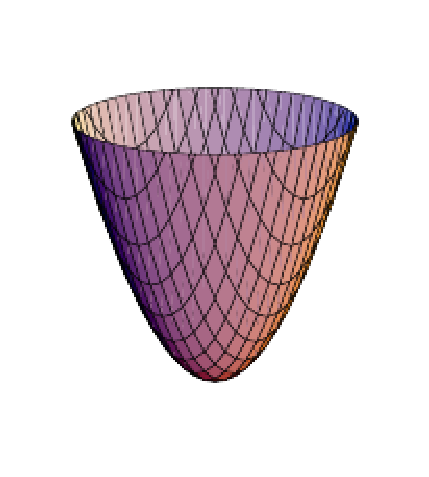
\includegraphics[scale=.9]{paraboloide}
&
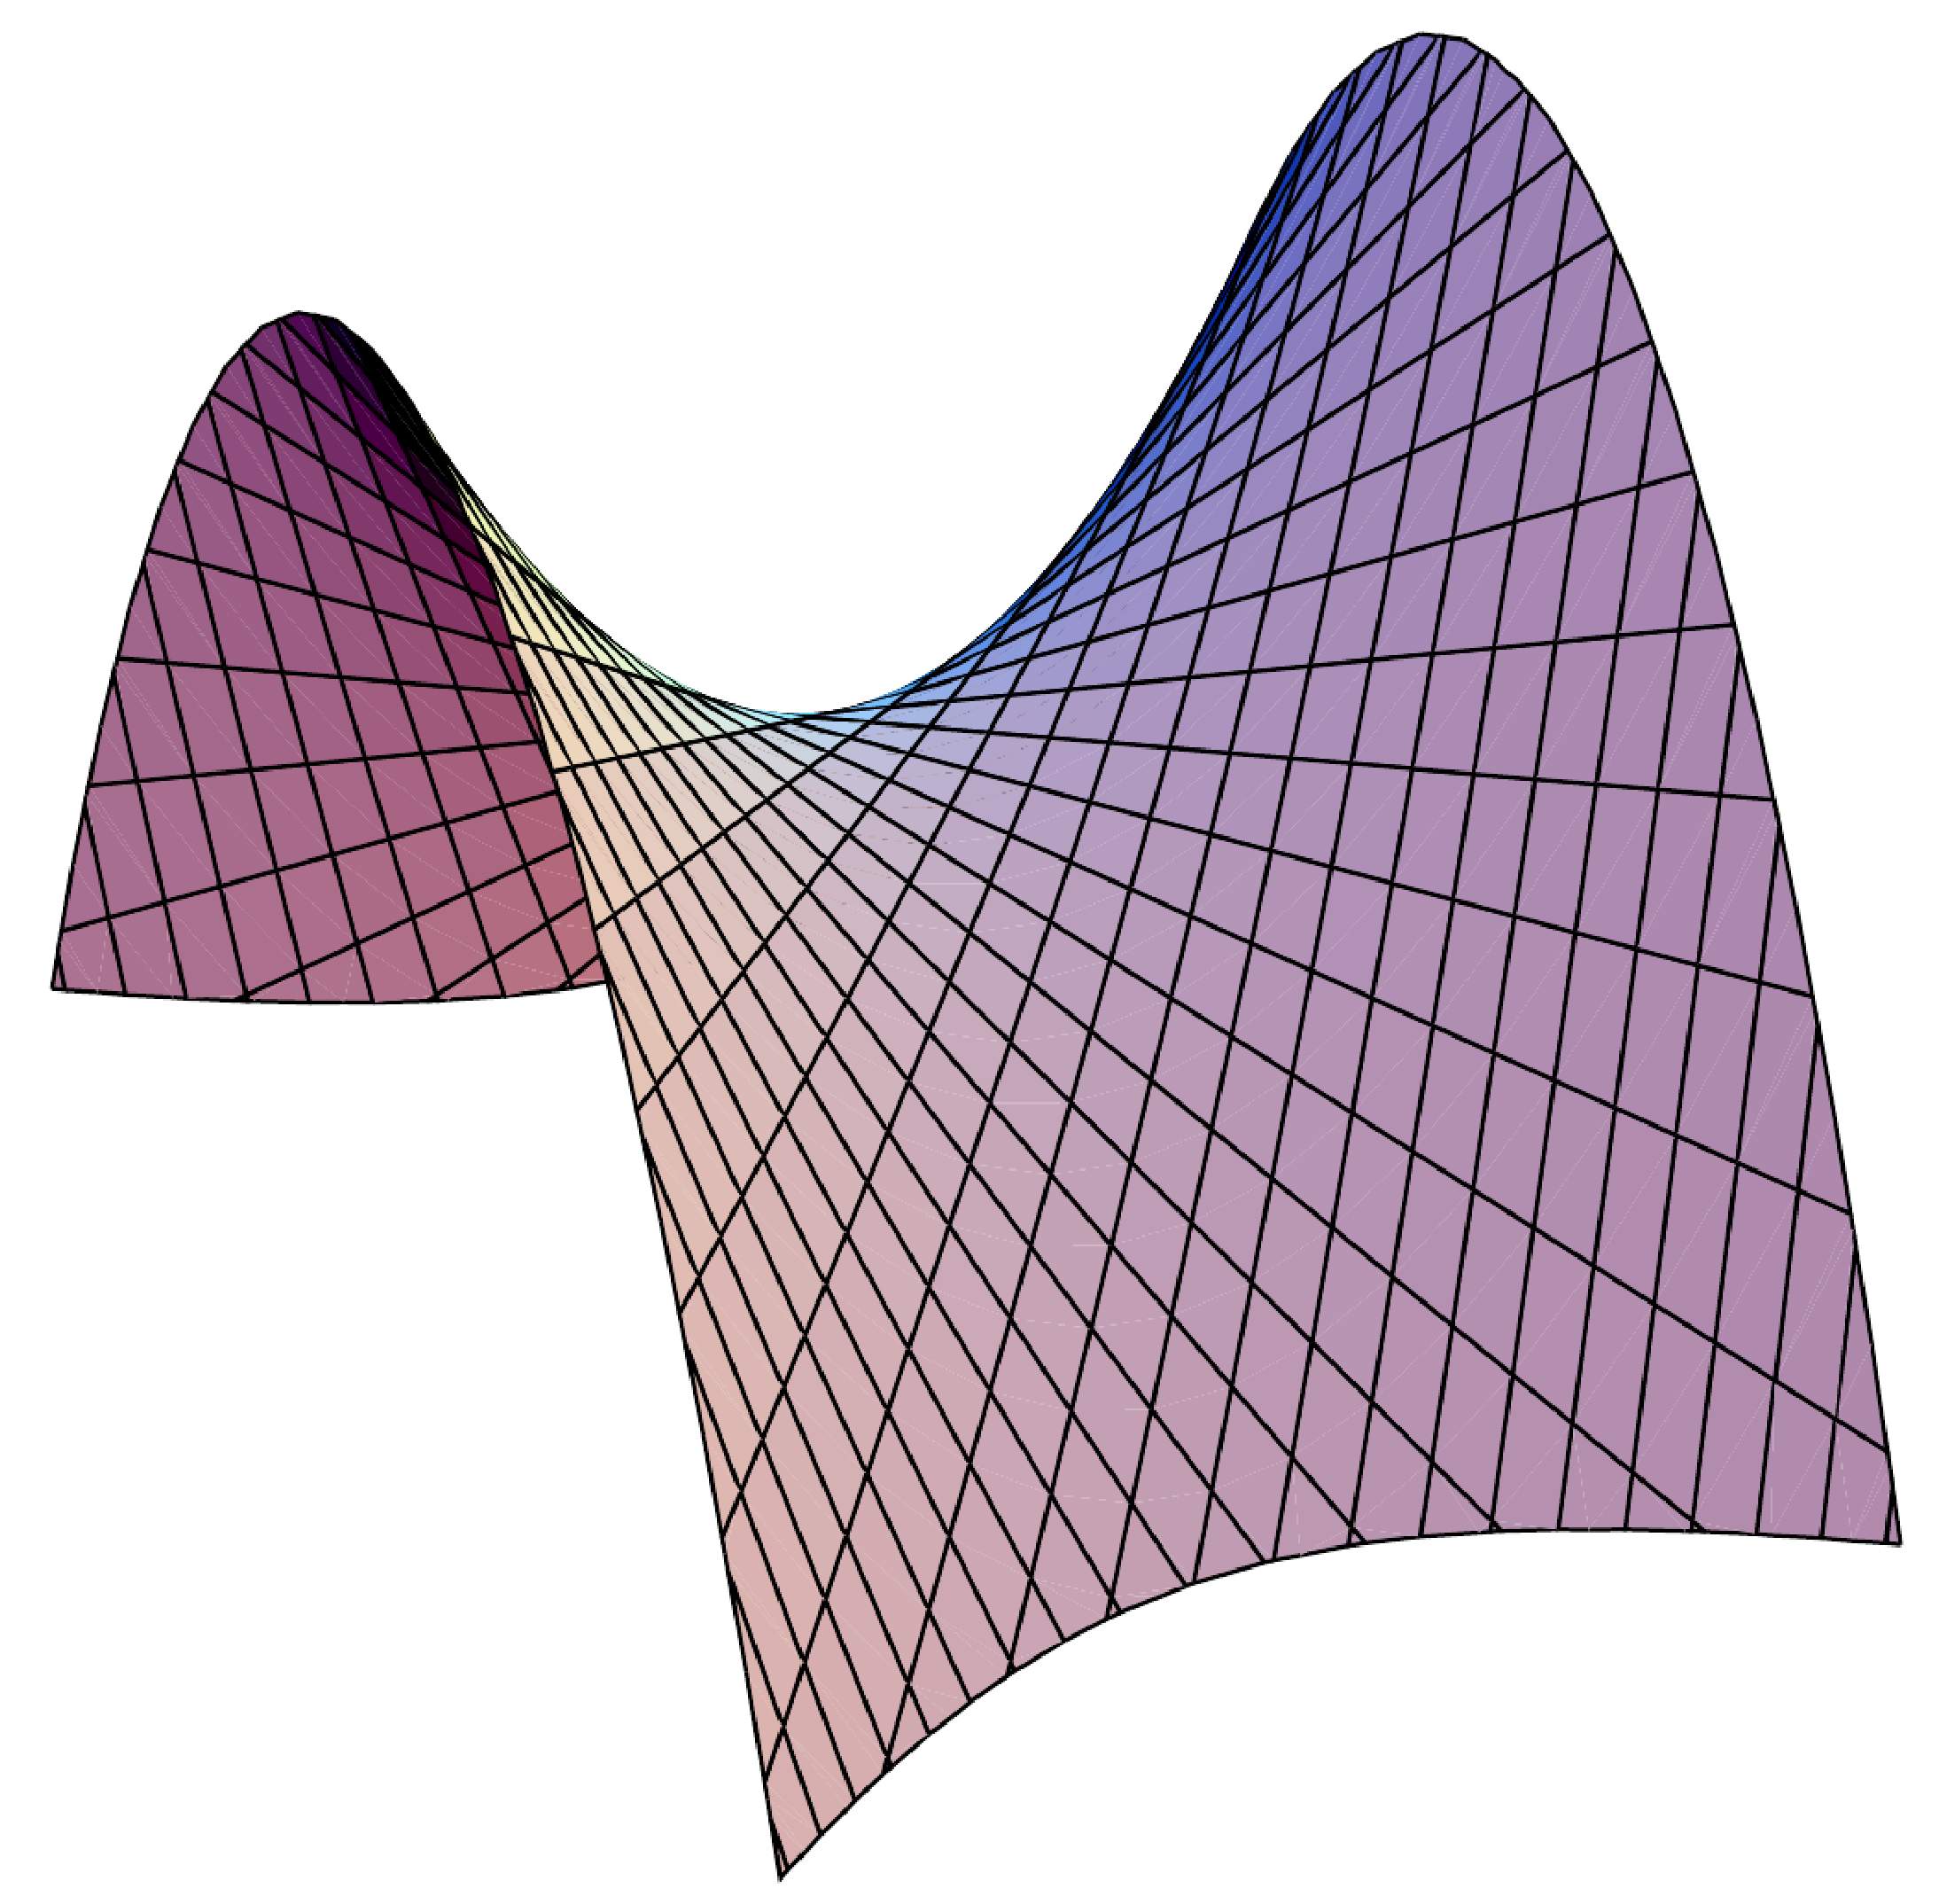
\includegraphics[scale=0.7]{hiperboloide_1_folha}
\end{array}
$
\caption{\textit{Parabolóide à esquerda e hiperbolóide de uma folha à direita.}}
\label{quadricas}
\end{figure}


Mais detalhes sobre a dedução da definição de uma quádrica podem ser encontrados em \cite{Hartley2004}, bem como outros exemplos além daqueles observados na figura \ref{quadricas}.\\

\subsubsection{A transformação de pontos e planos em $\mathbb{P}^3$}\label{sec.trans-pontos-planos-P3}

A transformação de pontos e planos em $\mathbb{P}^3$ é inteiramente análoga àquela argumentada na subseção \ref{sec.trans-proj-H} para pontos e retas em $\mathbb{P}^2$, pois assim como os pontos têm uma relação dual com retas em $\mathbb{P}^2$, os pontos também têm uma relação dual com planos em $\mathbb{P}^3$ e, como vimos, ambos têm a mesma representação em vetores homogêneos com quatro componentes. Assim, sob uma tranformação projetiva de pontos $\X'=H_{4\times4}\X$ temos que planos se transformam de acordo com

\begin{equation*}
\bpi'=H^{-\top}\bpi.
\end{equation*}







\subsubsection{Direções e o plano no infinito.}\label{sec.direcoes-plano-infinito}

O plano no infinito é denotado por $\bpi_\infty$, tem a forma canônica $\bpi_\infty=(0,0,0,1)^\top$ e é composto por pontos no infinito $D=(X_1,X_2,X_3,0)^\top$ que são as direções das retas contidas no espaço. No plano projetivo $\mathbb{P}^2$ duas retas paralelas se encontram num ponto no infinito, e analogamente, em  $\mathbb{P}^3$ dois planos paralelos se encontram numa reta que está contida no plano no infinito, e também, uma reta é paralela a outra reta (ou a um plano) se o ponto de interseção está no $\bpi_\infty$. O plano no infinito é invariável sob uma transformação afim.

De acordo com a subseção \ref{sec.trans-pontos-planos-P3} temos que a transformação projetiva de planos no espaço  $\mathbb{P}^3$ se dá pela fórmula $\bpi'=H^{-\top}\bpi$, assim podemos verificar porque um plano no infinito é invariante sob a tranformação afim. Conforme a subseção \ref{sec.hierarquia-transformacoes} vimos que a transformação afim é dada por 

\begin{equation*}
H_A=
\begin{bmatrix}
A&{\bf t}\\
{\bf 0}^\top&1
\end{bmatrix},
\end{equation*}
então

\begin{equation*}
H_A^{-\top}=
\begin{bmatrix}
A^{-\top}&{\bf 0}\\
-{\bf t}^\top A^{-\top}&1
\end{bmatrix},
\end{equation*}
e aplicando ao plano no infinito temos:

\begin{equation*}
\begin{array}{rcl}
\bpi'&=&H_A^{-\top}\bpi_\infty\\
&=&
\begin{bmatrix}
A^{-\top}&{\bf 0}\\
-{\bf t}^\top A^{-\top}&1
\end{bmatrix}\,
\begin{pmatrix}
0\\
0\\
0\\
1
\end{pmatrix}\\
&=&
\begin{pmatrix}
0&0&0&1
\end{pmatrix}^\top\\
&=&
\bpi_\infty.
\end{array}
\end{equation*}
Existem outros planos que podem ser invariáveis sob uma transformação afim menos específica, mas só o plano no infinito é invariante em uma transformação afim geral. Cabe resaltar que $\bpi_\infty$ é invariável apenas quando a transformação é aplicada ao conjunto, e não a pontos isolados pertencentes a esse plano.


\subsubsection{A cônica absoluta}\label{sec.con-absoluta}

A cônica absoluta é uma cônica (ponto) denotada por $\Omega_\infty$ e está contida no plano no infinito $\bpi_\infty$. Em coordenadas Euclidianas o plano no infinito tem definição $\bpi_\infty=(0,0,0,1)^\top$ (subseção \ref{sec.direcoes-plano-infinito}) e a cônica absoluta é definida através da equação matricial

\begin{equation*}
\X^\top\Omega_\infty\X=0,
\end{equation*} 
onde as componentes de $\X$ obedecem às restrições

\begin{equation*}
X_1^2+X_2^2+X_3^2=0\qquad\text{e}\qquad\,X_4=0.
\end{equation*}
De acordo com essas restrições e com esse sistema de coordenadas, e para satisfazer a equação matrical da cônica, podemos definir $\Omega_\infty=I_{3\times3}$, pois
\begin{equation*}
X_1^2+X_2^2+X_3^2=0\Leftrightarrow(X_1,X_2,X_3)\,I\,(X_1,X_2,X_3)^\top=0.
\end{equation*}

Da mesma forma que o plano no infinito é invariante sob uma transformação afim, a cônica absoluta é invariante sob uma transformação de similaridade. Já que a cônica absoluta está contida no plano no infinito, a transformação afim que mantem fixo esse plano também deverá manter invariável as coordenadas da cônica, sendo então a cônica absoluta invariável sob uma transformação afim
\begin{equation*}
H_A=
\begin{bmatrix}
A&{\bf t}\\
{\bf 0}^\top&1
\end{bmatrix}.
\end{equation*}
Aplicando a homografia afim $H_A$ aos pontos da cônica absoluta temos que as três primeiras componentes desses pontos são afetadas apenas pela submatriz $A_{3\times3}$,

\begin{equation*}
\begin{bmatrix}
A&{\bf t}\\
{\bf 0}^\top&1
\end{bmatrix}
\begin{pmatrix}
X_1\\
X_2\\
X_3\\
0
\end{pmatrix}
=
\begin{pmatrix}
A\,
\begin{pmatrix}
X_1\\
X_2\\
X_3
\end{pmatrix}\\
0
\end{pmatrix}.
\end{equation*}
Como vimos, essas três primeiras componentes são utilizadas na definição da cônica absoluta, e portanto $\Omega_\infty$ vai sofrer influência apenas de $A$ em tal transformação. 
De acordo com a tranformação de cônicas na subseção \ref{sec.trans-proj-H}, e com o fato de $\Omega_\infty$ ser invariável sob 
$H_A$, temos que $A^\top I A^{-1}=I$, assim

\begin{equation*}
\begin{array}{rcl}
I&=&A^{-\top}I\,A^{-1}\\
&=&A^{-\top}A^{-1}\qquad\text{tomando a inversa}\\
&=&A\,A^\top.
\end{array}
\end{equation*}
Desta forma percebemos que $A$ é uma matriz ortogonal (possivelmente com aplicação de escala), o que está de acordo com a definição de tranformação de similaridade $H_S$ conforme a subseção \ref{sec.hierarquia-transformacoes}.

\subsubsection{A quádrica dual absoluta}\label{sec.quadrica-dual-abs}
A quádrica dual absoluta é a dual degenerada da cônica absoluta $\Omega_\infty$, e é denotada por 
${\tt Q}^*_\infty$. Analogamente ao fato de que $C^*$ é o envelope das retas tangentes à cônica $C$ no ${\mathbb{P}}^2$, temos que, geometricamente, a quádrica dual absoluta é o envelope de todos os planos que são tangentes à cônica absoluta. Algebricamente, 
${\tt Q}^*_\infty$ é representada por uma matriz homogênea $4\times4$ e num sistema de coordenadas métrico tem a forma canônica

\begin{equation}\label{eq.quadrica-dual-abs}
{\tt Q}^*_\infty=
\begin{bmatrix}
1&0&0&0\\
0&1&0&0\\
0&0&1&0\\
0&0&0&0
\end{bmatrix}=
\begin{bmatrix}
I&{\bf 0}\\
{\bf 0}^\top&0
\end{bmatrix}.
\end{equation}
Para ver que os planos envelopados pela quádrica dual absoluta ${\tt Q}^*_\infty$ são tangentes à cônica absoluta $\Omega_\infty$, considere um plano $\bpi=({\bf v}, k)^\top$. Esse plano está no envelope definido por ${\tt Q}^*_\infty$ se, por definição, $\bpi^\top {\tt Q}^*_\infty\bpi=0$. Usando a matriz canônica na equação \ref{eq.quadrica-dual-abs} temos
\begin{equation}\label{eq.envelope-quadrica}
\begin{array}{rcl}
\bpi^\top {\tt Q}^*_\infty\bpi&=&
\begin{pmatrix}
{\bf v}^\top&k
\end{pmatrix}
\begin{bmatrix}
I&{\bf 0}\\
{\bf 0}^\top&0
\end{bmatrix}
\begin{pmatrix}
{\bf v}\\
k
\end{pmatrix}\\
&=&{\bf v}^\top {\bf v}\\
&=&0,
\end{array}
\end{equation}
onde ${\bf v}$ representa a reta de interseção do plano $\bpi$ com o plano no infinito $\bpi_\infty$. De acordo com as subseções \ref{sec.conica-dual} e \ref{sec.con-absoluta}, a reta ${\bf v}$ que pertence ao plano no infinito, é tangente à cônica absoluta se, e somente se, ${\bf v}^\top I\,{\bf v}=0$, o que está de acordo com a equação \ref{eq.envelope-quadrica}. Portanto, o envelope de ${\tt Q}^*_\infty$ é composto pelos planos que são tangentes à $\Omega_\infty$. 

Para constatar que ${\bf v}$ é a reta de interseção de $\bpi$ com $\bpi_\infty$, considere o sistema abaixo onde um ponto $\X$ pertence a esses dois planos. Esse ponto pertence a cada um dos planos se satisfaz o sistema

\begin{empheq}[left=\empheqlbrace]{align*}
\begin{pmatrix}
{\bf v}^\top&k
\end{pmatrix}
\begin{pmatrix}
X_1\\
X_2\\
X_3\\
X_4
\end{pmatrix}
=0\\
\bpi^\top_\infty
\begin{pmatrix}
X_1\\
X_2\\
X_3\\
X_4
\end{pmatrix}
=0.
\end{empheq}
Pela segunda equação, como $\bpi_\infty=(0,0,0,1)^\top$ (subseção \ref{sec.direcoes-plano-infinito}) temos que $X_4=0$ (o que já não era novidade). Substituindo $X_4=0$ na primeira equação e efetuando a multiplicação matricial, a constante $k$ desaparece multiplicada por zero e restará

\begin{equation*}
{\bf v}^\top
\begin{pmatrix}
X_1\\
X_2\\
X_3
\end{pmatrix}=0.
\end{equation*}
A última equação representa a equação de pertinência de um ponto a uma reta contida num plano conforme as subseções \ref{sec.reta} e \ref{sec.ponto}. 


\subsection{A câmera P}

A câmera é um dispositivo que transforma um cenário 3D referenciado por um sistema de coordenadas do mundo em uma imagem 2D no sistema de coordenadas da câmera. Algebricamente, a \textit{câmera} é modelada como uma transformação linear entre um ponto 3D no espaço e um ponto 2D no plano da imagem, representada por uma matriz $P_{3\times4}$ com algumas propriedades que realizam o mapeamento entre os pontos. Existem vários tipos de câmeras, mas para tratar das características básicas vamos utilizar o modelo buraco de alfinete, do inglês \textit{pinhole}.
\\
Esse tipo de câmera é uma composição de três mudanças de coordenadas, onde a matriz $P$ pode ser decomposta em:

\begin{equation*}
P = K \, [I|{\bf 0}]
\begin{bmatrix}
R&{\bf t}\\
\,\,{\bf 0}^\top &1
\end{bmatrix}
= K\,[R|{\bf t}],
\end{equation*}
tais que 

\begin{itemize}
\item a matriz $\begin{bmatrix}
R&{\bf t}\\
\,\,{\bf 0}^\top &1
\end{bmatrix}$
contendo os parâmetros extrínsecos transforma os pontos em coordenadas 3D no mundo para as coordenadas 3D da câmera.
\item a matriz $[I|{\bf 0}]$ aplica a projeção perspectiva passando um ponto na coordenada 3D da câmera para um ponto 2D em coordenadas normalizadas no plano da imagem.
\item a matriz $K$, matriz de calibração contendo os parâmetros intrínsecos, transforma pontos em coordenadas normalizadas no plano da imagem para as coordenadas na imagem ``final" (considerando mudanças como medida em pixels, por exemplo).  
\end{itemize}
Mais a frente vamos abordar cada um desses tópicos com mais detalhes.

Acompanhando pela figura \ref{camera} para fazermos a construção da câmera, consideramos (a princípio) o \textit{centro de projeção}, ou \textit{centro da câmera}, como a origem do espaço tridimensional Euclidiano, com o \textit{plano da imagem} ou \textit{plano focal} sendo $Z = f$, onde $f$ é a \textit{distancia focal} entre o plano da imagem e o centro de projeção. Assim, o plano da imagem é definido como $(x,y,f)^\top$ mas seu sistema de coordenadas é medido em pixels e é centralizado no canto inferior esquerdo da imagem. Por \textit{coordenadas normalizadas da imagem} nos referimos aos pontos $(x,y)^\top$ expressos como $(x,y,1)^\top$, (considerando que a câmera tenha distância focal unitária) no plano da imagem com relação ao sistema de coordenadas da câmera. O \textit{plano detector} fica em $(x,y,-f)^\top$. Como podemos obeservar na figura \ref{camera}, um ponto $\X$ no espaço 3D é mapeado a um ponto $\x$ no plano da imagem por uma reta que liga $\X$ ao centro de projeção, e intersecta o plano da imagem. O plano que passa pelo centro da câmera e é paralelo ao plano da imagem é chamado \textit{plano principal}, o plano $xy$ na figura \ref{camera}. O \textit{eixo principal} passa pelo centro da câmera e é perpendicular ao plano da imagem, onde a interseção desse eixo com o plano da imagem forma o \textit{ponto principal}, o qual pode ser pensado como a projeção do centro da câmera no plano da imagem.


\begin{figure}[!htb]
\centering
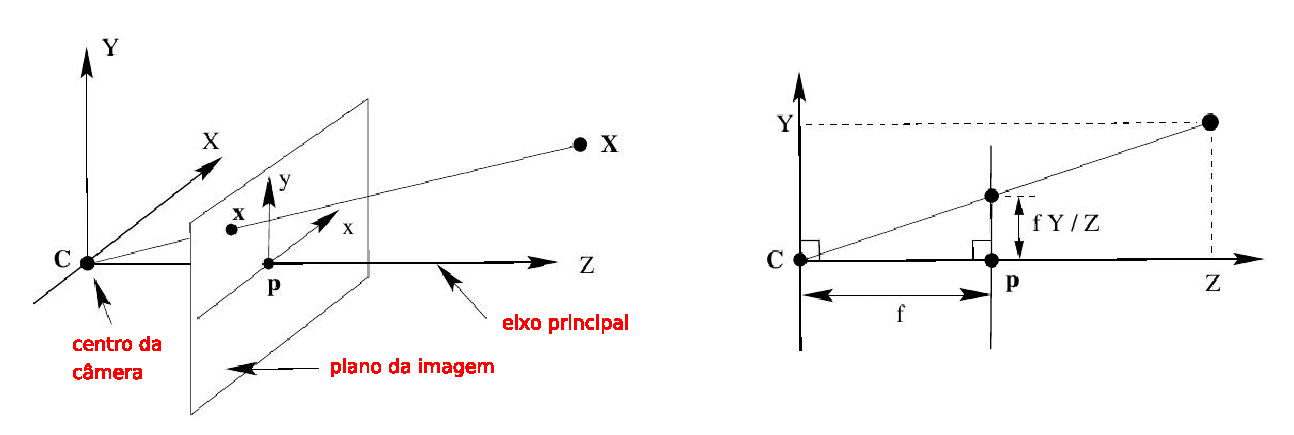
\includegraphics[scale=.75]{modelo_camera}
\caption{\textit{Visualização das características básicas de uma câmera como distância focal, eixo principal, plano da imagem, centro de projeção e o ponto principal {\bf P}.}}
\label{camera}
\end{figure}

Com vetores representados em coordenadas homogêneas, podemos expressar o mapeamento através de um operador linear, onde realizamos a multiplicação da matriz $P$, que representa a câmera, por um ponto no espaço, resultando num ponto na imagem conforme o esquema abaixo:

\begin{center}
$
\begin{array}{ccc}
\begin{pmatrix}
fX\\
fY\\
Z
\end{pmatrix} = 
&
\begin{bmatrix}
f& & &0\\
 &f& &0\\
 & &1&0
\end{bmatrix}
&
\begin{pmatrix}
X\\
Y\\
Z\\
1
\end{pmatrix}
\end{array}
$
\end{center}

Nessa matriz temos que $f$ é a distância focal (entre o centro da câmera e o plano da imagem), e o vetor de coluna de zeros à direita representa as coordenadas do centro da câmera, que nesse caso está na origem do sistema. Essa matriz pode ser desmembrada da seguinte maneria: uma matriz diagonal $diag(f,f,1)$ multiplicada pela matriz $[I|{\bf 0}]$, onde $I$ é uma matriz identidade $3\times3$ e ${\bf 0}$ é um vetor coluna de zeros. Compactamente, podemos escrever a ultima relaçao como:

\begin{center}
$\x = diag(f,f,1)\,[I|{\bf 0}]\,\X$,
\end{center}
onde $diag(f,f,1)\,[I|{\bf 0}]$ é a matriz da câmera para o modelo \textit{pinhole}.

Nessa dedução, consideramos que o ponto principal  coincide com a origem do plano da imagem, mas na prática isso pode não acontecer. Dessa forma, devemos acrescentar as coordenadas do ponto na construção da matriz da câmera. Sendo $(p_x,p_y)$ as coordenadas do ponto principal, desejamos o seguinte mapeamento (em coordenadas não homogêneas):

\begin{center}
$(X,Y,Z)^\top \rightarrow (\frac{f\,X}{Z}+p_x\,,\,\frac{f\,Y}{Z}+p_y)$,
\end{center}
o qual nos fornece a seguinte relação de projeção em coordenadas homogêneas:

\begin{center}
$
\begin{array}{ccc}
\begin{pmatrix}
f\,X + Z\,p_x\\
f\,Y + Z\,p_y\\
Z
\end{pmatrix}=
&
\begin{bmatrix}
f& &p_x&0\\
 &f&p_y&0\\
 & &1&0
\end{bmatrix}
\begin{pmatrix}
X\\
Y\\
Z\\
1
\end{pmatrix}
\end{array}
$
\end{center}
Definindo a notação

\begin{center}
$
\begin{array}{cc}
K = & \begin{bmatrix}
      f& &p_x\\
       &f&p_y\\
       & &1
      \end{bmatrix}, 
\end{array}
$
\end{center}
a relação de projeção assume a forma


\begin{equation}\label{eq.camera-incompleta}
\x=K\,[I|{\bf 0}]\,\X_{\textit{cam}},
\end{equation}
onde $K$ é denominada matriz de calibração da câmera, a qual resume os parâmetros internos da mesma, e $\X_{\textit{cam}}$ enfatiza que o ponto 3D está escrito no sistema de coordenadas da câmera.

A matriz de calibração $K$ ainda não está completa, pois o sistema de coordenadas do plano da imagem é medido em pixels, que podem ser não quadrados, e além disso os eixos cartesianos desse sistema podem ser não ortogonais. Assim, vamos inserir mais dois parâmetros para definir a medição em pixels e mais um parâmetro para definir o ângulo de inclinação entre os eixos cartesianos.

Sendo $m_x$ e $m_y$ a quantidade de pixels nas direções $x$ e $y$, respectivamente, a transformação para a coordenadas em pixels se dá pela multiplicação da matriz $diag(m_x,m_y,1)$ à esquerda da matriz $K$,
\begin{equation*}
\begin{bmatrix}
m_x&0&0\\
0&m_y&0\\
0&0&1
\end{bmatrix}      
\begin{bmatrix}
f& &p_x\\
&f&p_y\\
& &1
\end{bmatrix}
=
\begin{bmatrix}
\alpha_x&0&x_0\\
0&\alpha_y&y_0\\
0&0&1
\end{bmatrix}
\end{equation*}
onde $\alpha_x=m_x\,f$, $\alpha_y=m_y\,f$ representa a distância focal em termos das dimensões dos pixels. Similarmente, $x_0=m_x\,p_x$ e $y_0=m_y\,p_y$ são as coordenadas do ponto principal medidas em pixels. Para completar a generalidade, acrescentamos o parâmetro $s$, referente à inclinação entre os eixos, na matriz
\begin{equation*}
K=
\begin{bmatrix}
\alpha_x&s&x_0\\
0&\alpha_y&y_0\\
0&0&1
\end{bmatrix}.
\end{equation*}






Até aqui temos expressado o ponto $\X$ no espaço em relação às coordenadas da câmera, assumindo que o centro da câmera está situado na origem do sistema de eixos, o qual recebe o nome de sistema de coordenadas da câmera. Mas na maioria das vezes esse não é o caso, portanto desejamos fazer o mapeamento de um ponto 3D cujo as coordenadas estejam expressas com relação a um sistema de coordenadas qualquer, chamado sistema de coordenadas do mundo. Portanto, vamos continuar completando a matriz $P$ para mapear pontos no sistema de coordenadas do mundo.

Considerando o sistema de coordenadas do mundo, denotaremos um ponto nesse sistema, em coordenadas não homogêneas, por $\overline{\X}$, e o mesmo ponto no sistema de coordenadas da câmera será denotado por $\overline{\X}_{\textit{cam}}$. A transferência de sistemas de coordenadas é feita através da relação $\overline{\X}_{\textit{cam}}=R\,(\overline{\X}-\overline{\bf C})$, onde $\overline{\bf C}$ representa o centro da câmera no sistema de coordenadas do mundo e $R$ representa uma matriz de rotação $3\times3$. Passando os vetores para coordenadas homogêneas, podemos aplicar a rotação no vetor $\overline{\bf C}$, do centro da câmera, e inseri-lo na quarta coluna da matriz escrevendo a relação

\begin{center}
$
\begin{array}{ccc}
\X_{\textit{cam}}=
&
\begin{bmatrix}
R&-R\,\overline{\bf C}\\
\,\,{\bf 0}^\top&\,\,1
\end{bmatrix}
&
\begin{pmatrix}
X\\
Y\\
Z\\
1
\end{pmatrix},
\end{array}
$
\end{center} 
onde podemos escrever

\begin{center}
$
\begin{array}{cccc}
R=
&
\begin{bmatrix}
a&b&c\\
d&e&f\\
g&h&i
\end{bmatrix}
&
\qquad\text{e}\qquad
&
-R\,\overline{\bf C}=(t_1,t_2,t_3)^\top,
\end{array}
$
\end{center}
e a relação acima fica:
\begin{center}
$
\begin{array}{ccc}
\X_{\textit{cam}}=
&
\begin{bmatrix}
a&b&c&t_1\\
d&e&f&t_2\\
g&h&i&t_3\\
0&0&0&\,1
\end{bmatrix}
&
\begin{pmatrix}
X\\
Y\\
Z\\
1
\end{pmatrix}.
\end{array}
$
\end{center}
Substituindo $\X_{\textit{cam}}$ em \ref{eq.camera-incompleta}, obtemos

\begin{center}
$
\begin{array}{ccccc}
\x=
&
\begin{bmatrix}
\alpha_x&s&x_0\\
0&\alpha_y&y_0\\
0&0&1
\end{bmatrix}&
\begin{bmatrix}
1&0&0&0\\
0&1&0&0\\
0&0&1&0
\end{bmatrix}
&
\begin{bmatrix}
a&b&c&t_1\\
d&e&f&t_2\\
g&h&i&t_3\\
0&0&0&\,1
\end{bmatrix}
&
\begin{pmatrix}
X\\
Y\\
Z\\
1
\end{pmatrix},
\end{array}
$
\end{center}
multiplicando a segunda e terceira matrizes,
\begin{center}
$
\begin{array}{cccc}
\x=
&
\begin{bmatrix}
\alpha_x&s&x_0\\
0&\alpha_y&y_0\\
0&0&1
\end{bmatrix}&
\begin{bmatrix}
a&b&c&t_1\\
d&e&f&t_2\\
g&h&i&t_3
\end{bmatrix}
&
\begin{pmatrix}
X\\
Y\\
Z\\
1
\end{pmatrix},
\end{array}
$
\end{center}
que pode ser escrita de forma resumida como
\begin{center}
$
\x=K\,[R|{\bf t}]\,\X,
$
\end{center}
com ${\bf t}=(t_1,t_2,t_3)^\top$ denominado vetor de translação.

Acabamos de incluir todos os parâmetros na matriz $P=K\,[R|{\bf t}]$, para o mapeamento de um ponto 3D homogêneo no sistema de coordenadas do mundo em seu respectivo ponto 2D no plano da imagem, no sistema de coordenadas da imagem. Temos cinco parâmetros internos na matriz de calibração $K$, $(\alpha_x,\alpha_y,s,p_x,p_y)$, três parâmetros externos na matriz de rotação $R$, apesar de suas nove entradas, e mais três parâmetros externos no vetor de translação totalizando 11 graus de liberdade. Repare que, tendo a matriz $P$ dimensão $3\times4$, ela possui 12 componentes e, usando uma para determinar a escala, sobram exatamente os 11 graus de liberdade, e a câmera $P$ é chamada câmera de \textit{projeção finita}.

\subsubsection*{A matriz de calibração K}

A intenção nesta seção é mostrar qual é a natureza de cada um dos parâmetros internos da matriz de calibração. Para isso, vamos resolver o problema de transferir um ponto qualquer no espaço (em coordenadas não homogêneas) para o plano da imagem na câmera, conforme encontrado em \citep{tese-fabbri}.

\paragraph*{Problema:} Dado um ponto 3D $p^w = (x^w,y^w,z^w)^\top$ em coordenadas do mundo e sendo $(\uu,\vv)$ as coordenadas do ponto na imagem da câmera, quais os valores de $(\uu,\vv)$?

Primeiramente, vamos transformar o ponto em coordenadas do mundo para as coordenadas da câmera, $p = (x,y,z)^\top$ e
\begin{align*}
p = R p^w + T
\end{align*}
onde $R$ e $T$ são parâmetros extrínsecos. Agora, vamos projetar o ponto para o plano imagem normalizada usando similaridade de triângulos
\begin{empheq}[left=\empheqlbrace]{align*}\label{eq:normalized:coords}
\tilde x = \frac{x}{z}\\
\tilde y = \frac{y}{z}
\end{empheq}

Depois dessa projeção, vamos aplicar os parâmetros internos para obtermos as coordenadas finais da imagem. O primeiro passo é incluir a distância focal.
\begin{empheq}[left=\empheqlbrace]{align*}
\tilde x &= f\frac{x}{z}\\
\tilde y &= f\frac{y}{z}
\end{empheq}
Então converter para pixels:
\begin{empheq}[left=\empheqlbrace]{align*}
\tilde x_{pix} &= s_\uu f\frac{x}{z}\\
\tilde y_{pix} &= s_\vv f\frac{y}{z},
\end{empheq}
onde $s_\uu$ e $s_\vv$ é a quantidade de pixels por unidade de comprimento nas direções $\uu$ e $\vv$, respectivamente. Como podemos ver, $f$ tem efeito similar a $s_\uu$ e $s_\vv$. Seria suficiente mantermos apenas dois parâmetros, digamos $f$ e a razão de aspecto $\frac{s_\uu}{s_\vv}$, mas vamos manter os três parâmetros por enquanto.
%
%
Em seguida, fazemos a translação para o ponto inferior esquerdo da imagem usando $(t_{\tilde \uu},t_{\tilde \vv})$, que são as coordenadas do ponto principal em relação ao inferior esquerdo da imagem:
\begin{empheq}[left=\empheqlbrace]{align*}
\tilde \uu &= s_\uu f\frac{x}{z} + t_{\tilde \uu}\\
\tilde \vv &= s_\vv f\frac{y}{z} + t_{\tilde \vv},
\end{empheq}
e convertemos para o sistema de coordenadas em função de um ângulo $\theta$ entre os eixos, pois os eixos podem ser não ortogonais. Observe na figura \ref{skew} a conversão das coordenadas de um ponto $Q$ qualquer:

\begin{figure}[!htb]
\centering
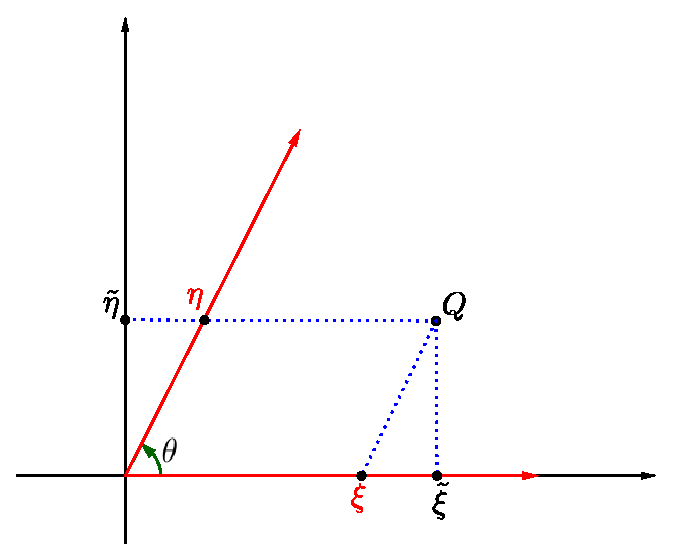
\includegraphics[scale=1]{skew}
\caption{\textit{Transformação das coordenadas de um ponto no plano com eixos perpendiculares para um plano com eixos relacionados por um ângulo $\theta$ qualquer.}}
\label{skew}
\end{figure}

\begin{empheq}[left=\empheqlbrace]{align*}
\tilde \uu &= \uu + \vv \, \cos\,\theta
\\
\tilde \vv &= \vv \, \sin\,\theta
\end{empheq}
Isolando as variáveis do sistema de coordenadas com ângulo genérico temos:


\begin{empheq}[left=\empheqlbrace]{align*}
\uu &= \tilde \uu - \tilde \vv \cot\theta \\
\vv &= \tilde \vv \,\csc\, \theta
\end{empheq}
os quais fornecem
\begin{empheq}[left=\empheqlbrace]{align*}\label{eq:projection:explicit}
\uu &= \overbrace{s_\uu f}^{\alpha_\uu}\frac{x}{z} + \overbrace{(-\cot\theta\, s_\vv
f)}^{\sigma_\theta} \frac{y}{z} + \overbrace{t_{\tilde \uu} - \cot\theta\, t_{\tilde \vv}}^{\uu_0}\\
%
\vv &= \underbrace{s_\vv f\,\csc\,\theta}_{\alpha_\vv} \frac{y}{z}+
\underbrace{\csc\,\theta\, t_{\tilde \vv}}_{\vv_0}
\end{empheq}
Assim, a transformação de um ponto expresso nas coordenadas da câmera para a imagem é feita usando cinco parâmetros da matriz de calibração
\begin{equation*}
K = \begin{bmatrix}
\alpha_\uu & \sigma & \uu_o\\
0 &\alpha_\vv &  \vv_o\\
0 & 0 &  1
\end{bmatrix}.
\end{equation*}
A fórmula acima explicita a interpretação de cada um desses parâmetros.


\begin{table}
\begin{center}
\begin{tabular}{c l} 
\textbf{Variáveis Livres} & \textbf{Descrição}\\
3	 & rotação \\
3	 & translação \\
2	 & mudança de escala em $x,y$\\
1	 & distância focal (pode ser incorporada como escala)\\
2	 & ponto principal\\
1	 & ângulo entre os eixos \\
6  & total extrinsecos\\
6  & total intrinsecos\\
12 & total\\
11 & total único (distância focal para fixar escala)
\end{tabular}
\end{center}
\caption{Resumo dos parâmetros da câmera.}
\end{table}

\subsection{A ação projetiva de uma câmera $P$}
Nesta subseção iremos verificar como se dá a projeção aplicada por uma câmera $P$ em planos, retas, cônicas e quádricas.


\subsubsection*{Ação projetiva de $P$ em planos}
A equação de projeção $\x=P\,\X$ é uma transformação de um ponto em coordenadas 3D no sistema de coordenadas do mundo para pontos 2D no sistema de coordenadas do plano da imagem na câmera e, por conta das características invariantes sob transformação projetiva, temos a liberdade para escolher o sistema de coordenadas do mundo. Assim, suponha que tal sistema de coordenadas seja posicionado de forma que o plano $xy$ corresponda ao plano $\bpi$, conforme ilustrado na figura \ref{fig.projecao-planos-retas}. Desta forma, pontos no espaço que pertençam ao plano $\bpi$ terão a componente $X_3=0$, e a ação de uma câmera $P$ nesses pontos é dada por

\begin{equation*}
\begin{array}{rcl}
\x&=&P\,\X\\
&=&
\begin{pmatrix}
{\bf p_1}&{\bf p_2}&{\bf p_3}&{\bf p_4}
\end{pmatrix}
\begin{pmatrix}
X_1\\
X_2\\
0\\
1
\end{pmatrix}\\
&=&
\begin{pmatrix}
{\bf p_1}&{\bf p_2}&{\bf p_4}
\end{pmatrix}
\begin{pmatrix}
X_1\\
X_2\\
1
\end{pmatrix},
\end{array}
\end{equation*}
onde ${\bf p_i}$ são as colunas da matriz $P$. Assim, a transformação de um ponto $\X_\pi=(X_1,X_2,1)^\top\in\bpi$ para um ponto na imagem é, em geral, uma homografia planar, ou uma transformação projetiva de plano a plano $\x=H\,\X_\pi$.


\begin{figure}[htb!]
\centering
\subfloat[]{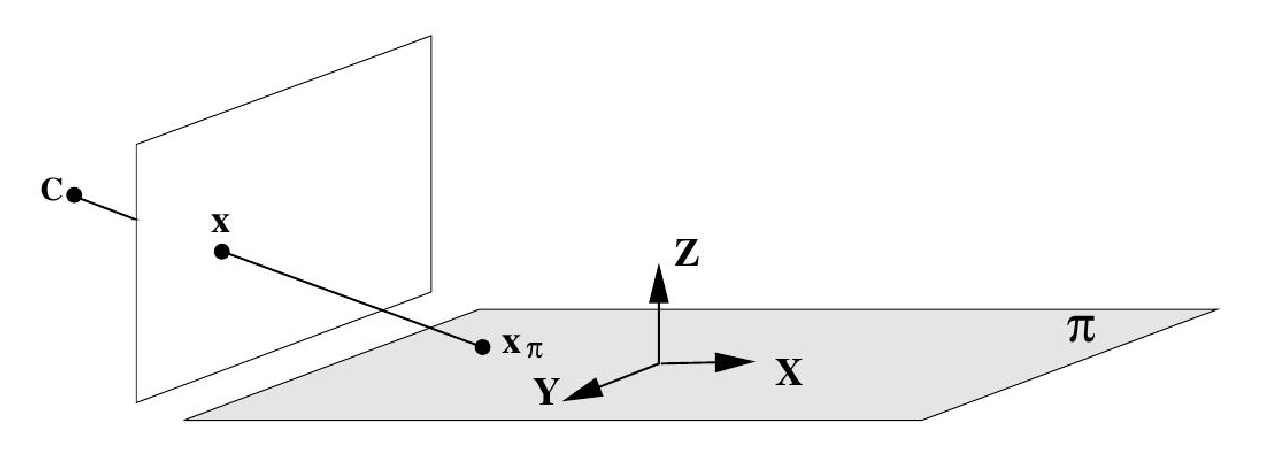
\includegraphics[scale=.5]{projecao-planos}}
\quad
\subfloat[]{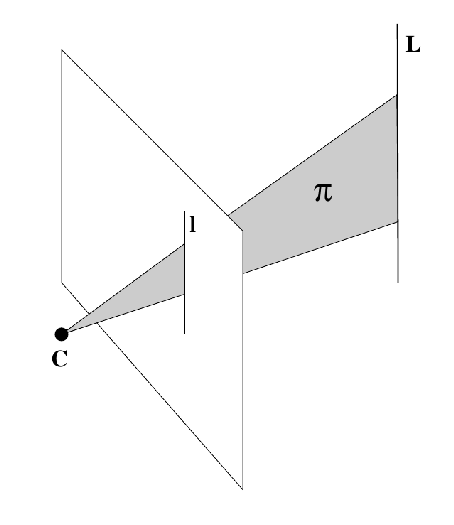
\includegraphics[scale=.5]{projecao-retas}}
\caption{({\tt a})\textit{Transformação projetiva de plano a plano induzida pela câmera $P$.}\,\,({\tt b})\textit{Plano $\bpi$ retroprojetado por uma reta $\lightrgb$ no plano da imagem através da câmera $P$.}}
\label{fig.projecao-planos-retas}
\end{figure}

\subsubsection{A ação projetiva de $P$ em retas}\label{sec.proj.retas}
Geometricamente, como podemos ver na figura \ref{fig.projecao-planos-retas}, uma reta ${\bf L}$ no espaço 3D junto com o centro $\C$ da câmera definem um plano. A interseção desse plano com o plano da imagem é uma reta $\lightrgb$, que é a imagem da reta ${\bf L}$ no espaço. Algebricamente, considere uma reta ${\bf L}$ parametrizada por $\lambda$ passando pelos pontos ${\bf A}$ e ${\bf B}$, onde cada ponto nessa reta é dado por $\X(\lambda)={\bf A}+(\lambda)\,{\bf B}$. Considere ainda, ${\bf a}$ e ${\bf b}$ sendo as imagens dos pontos ${\bf A}$ e ${\bf B}$ sob a ação da câmera $P$. Aplicando a projeção da câmera $P$ aos pontos da reta ${\bf L}$ temos

\begin{equation*}
\begin{array}{rcl}
\x(\lambda)&=&P\,\X(\lambda)\\
&=&P({\bf A}+(\lambda)\,{\bf B})\\
&=&P\,{\bf A}+(\lambda)\,P\,{\bf B}\\
&=&{\bf a}+(\lambda)\,{\bf b},
\end{array}
\end{equation*}
onde cada $\x$ em função de $\lambda$ pertence à reta passando por ${\bf a}$ e ${\bf b}$ no plano da imagem.  

\subsubsection*{Retroprojeção de retas.}
Geometricamente, a retroprojeção de retas é o conjunto de pontos no espaço pertencentes a um plano, o qual é definido pelo centro da câmera e uma reta na imagem, como na figura \ref{fig.projecao-planos-retas}. Algebricamente, sendo a reta na imagem denotada por $\lightrgb$ e a camera por $P$, o plano retroprojetado é $P^\top\lightrgb$. De fato, um ponto $\X$ no espaco é projetado na imagem como $\x=P\,\X$, e esse ponto pertence a reta $\lightrgb$ na imagem se $\x^\top\lightrgb=0$ ou, substituindo, $(P\,\X)^\top\lightrgb=0$. Então, aplicando a transposta, $\X^\top P^\top\lightrgb=0$ e $P^\top\lightrgb$ é tomado como o plano que contém o ponto $\X$ no espaço. Assim, tal plano é a retroprojeção da reta $\lightrgb$.  

\subsubsection*{A ação projetiva de $P$ em cônicas}
Um cone é uma quádrica degenerada, representada por uma matriz $4\times4$ que não tem posto completo, e é denotada por ${\tt Q}_{co}$.

\subsubsection*{Retroprojeção de cônicas.}
Uma cônica retroprojeta um cone ${\tt Q}_{co}$ que, neste caso, tem o vértice coincidindo com o centro da câmera, onde esse vértice é o vetor nulo da matriz $4\times4$ que representa o cone. Uma cônica retroprojeta um cone de acordo com 

\begin{equation*}
{\tt Q}_{co}=P^\top C\,P
\end{equation*}
pois, um ponto $\X$ no espaço é projetado na imagem na forma $\x=P\,\X$, e $\x\in C$ se satisfaz a equação $\x^\top C\,\x=0$. Substituindo $\x$ na equação da cônica temos $(P\,\X)^\top C\,P\,\X=0$, e aplicando a transposição, $\X^\top P^\top C\,P\,\X=0$. O ponto $\X$ é projetado na cônica $C$ se , se e somente se, $\X\in {\tt Q}_{co}$, que deve ser definida como ${\tt Q}_{co}=P^\top C\,P$. Assim, um cone é a retroprojeção de uma cônica, e repare que não há a projeção direta de uma cônica, já que uma cônica é definida por uma matriz $3\times3$ e a matriz da câmera é $3\times4$.

\subsubsection{A ação projetiva de $P$ em quádricas}\label{sec.proj-quadricas}
Para tratarmos desse assunto, primeiramente precisamos definir alguns conceitos.

\subsubsection*{Contorno gerador e contorno aparente.}
Na formação da imagem de uma superfície, os raios de luz passando pelo centro da câmera são tangentes à essa superficie em 3D. O contorno dessa superfície nesses pontos de tangência é transformado num contorno no plano da imagem conforme a figura \ref{fig.cont-gerador-aparente}. O contorno da superfície é denominado \textit{contorno gerador} e denotado por ${\bf \Gamma}$, o contorno formado na imagem é chamado \textit{contorno aparente} e denotado por ${\bf \gamma}$. Vale ressaltar que o contorno gerador depende das posições do centro da câmera e da própria superfície, e não depende do plano da imagem.  

\begin{figure}[htb!]
\centering
\subfloat[]{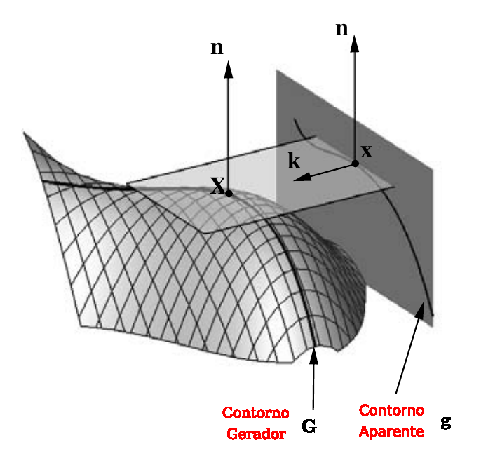
\includegraphics[scale=.94]{contorno-gerador-aparente}}
\subfloat[]{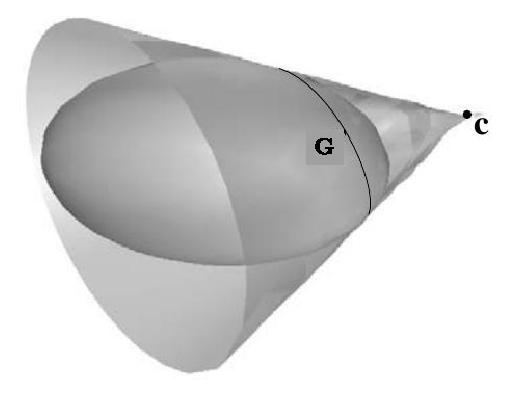
\includegraphics[scale=.94]{superficie-lisa}}
\caption{\textit{$({\tt a})\,$O contorno aparente é a imagem do contorno gerador, onde essa imagem fica definida pelas retas através do centro da câmera que são tangentes aos pontos no contorno gerador.$\,\,({\tt b})\,$ Uma quádrica tangenciada por um cone que é o formado pelo conjunto de retas passando pelo centro da câmera, onde tais retas são tangentes ao contorno gerador ${\bf \Gamma}$. }}
\label{fig.cont-gerador-aparente}
\end{figure}

\subsubsection*{Projeção de quádricas.}
A quádrica é uma superfície lisa  e o seu contorno gerador produz um contorno aparente no plano da imagem, através dos raios retroprojetados pelos pontos do contorno aparente e passando pelo centro da câmera, conforme um exemplo na figura \ref{fig.cont-gerador-aparente}. Assim, o contorno gerador é uma cônica e sob uma transformação projetiva o contorno aparente também é uma cônica na imagem. Como estamos usando relações de tangência aos contornos gerador e aparente, será necessária a utilização da quádrica dual	${\tt Q}^*$, já que por definição a equação que representa a quádrica dual fica definida pelos planos $\bpi$ que são tangentes ao contorno gerador na quádrica ${\tt Q}$. Portanto, a equação da quádrica dual é dada por
\begin{equation*}
\bpi^\top {\tt Q}^*\bpi=0.
\end{equation*}
Sejam $\lightrgb$ as retas tangentes à conica $C$ na imagem (contorno aparente), onde a cônica dual define a relação $\lightrgb^\top C^*\lightrgb=0$. Essas retas $\lightrgb$ retroprojetam planos definidos por $\bpi=P^\top\lightrgb$ (subseção \ref{sec.proj.retas}), que são tangentes à quádrica ${\tt Q}$ e satisfazem a relação $\bpi^\top {\tt Q}^*\bpi=0$. Substituindo o plano nessa última relação temos

\begin{equation*}
\begin{array}{rcl}
\bpi^\top {\tt Q}^*\bpi&=&(P^\top\lightrgb)^\top {\tt Q}^*P^\top\lightrgb\\
&=&\lightrgb^\top P\,{\tt Q}^*P^\top\lightrgb\\
&=&\lightrgb^\top C^*\lightrgb\\
&=&0,
\end{array}
\end{equation*}
onde tomamos $C^*=P\,{\tt Q}^*P^\top$, a imagem da quádrica sob a projeção $P$.

\subsection{A geometria bifocal}

\subsubsection*{A geometria epipolar}

Considere um cenário com um ponto $\X$ no espaço 3D e dois planos que contêm as imagens $\x$ e $\x'$ desse ponto $\X$. Considere ainda um plano $\bpi$ que contém esse ponto $\X$ e os dois centros de projeção (ou centro da câmera) das duas câmeras, denotados por $\C$ e $\C'$. A geometria epipolar se constitui nas relações existentes entre as interseções desse plano $\bpi$ com os dois planos das imagens observado na figura \ref{fig.geo-epipolar}. Sendo $\x$ a imagem 2D de $\X$ no primeiro plano de imagem, a construção desse cenário é motivada pela busca de $\x'$, também 2D, que seja correspondente a $\x$, onde $\x'$ é a imagem de $\X$ no segundo plano de imagem. Ou seja, existem as matrizes que promovem a ação de cada câmera onde $\x=P\,\X$ e $\x'=P'\,\X$, e quando isso acontece dizemos que os pontos são {\it pontos correspondentes}, e denotamos por $\x\leftrightarrow\x'$ (já definidos anteriormente). Podemos observar que $\x$ e $\x'$ retroprojetam duas retas definidas por $\C$ e $\C'$, onde esses retas pertencem a $\bpi$ e se interceptam em $\X$. Essa propriedade é essencial para nos auxiliar a definir as correspondências entre os pontos nas duas imagens. 

A \textit{reta base} é a reta que passa pelo centro de cada câmera $\C$ e $\C'$. O plano $\bpi$ fica determinado pela reta base e pela reta definida por $\x$ e $\C$. A interseção de $\bpi$ com o segundo plano de imagem define uma reta chamada \textit{reta epipolar}, que é a imagem na segunda visão da reta retroprojetada por $\x$. Ou seja, dadas duas imagens de uma cena, para cada ponto numa imagem vai existir uma reta epipolar correspondente na outra imagem. Pela construção, sabemos que $\x'\in\bpi$ e pertence ao plano da segunda imagem, portanto $\x'$ pertence à reta epipolar que será denotada por $\lightrgb'$. Assim, nossa busca pela correspondência de $\x$ se restringirá a uma busca numa reta e não a uma busca em todo o plano de imagem da segunda câmera. 
\begin{equation*}
\x\rightarrow\lightrgb'
\end{equation*}
A imagem do centro de projeção da primeira câmera na segunda fotografia é denominada \textit{epipolo} e denotada por $\e'$. Analogamente, a imagem de $\C'$ na primeira fotografia também é chamada epipolo e é denotada por $\e$.
O plano $\bpi$ é denominado \textit{plano epipolar} e num sistema com duas vistas temos vários planos epipolares definidos por um único parâmetro, e que formam o feixe de planos girando em torno da reta base.

\begin{figure}[!htb]
\centering
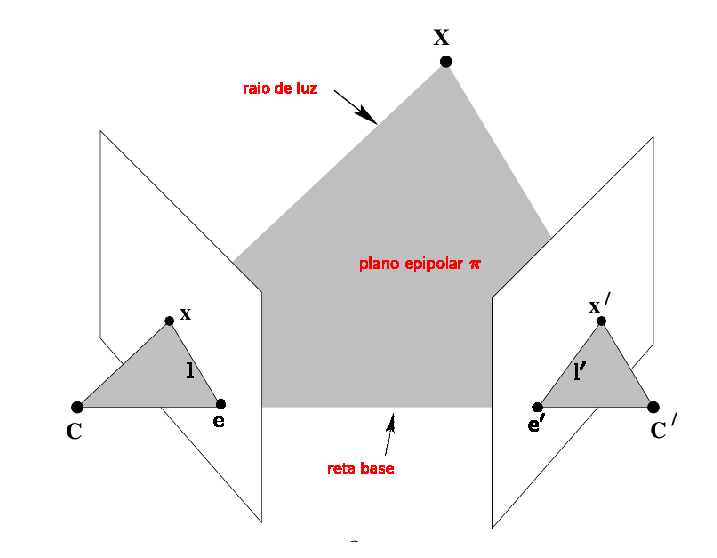
\includegraphics[scale=1.2]{geometria-epipolar}
\caption{\textit{O plano epipolar contém o ponto $\X$, os centros das câmeras, e define as retas epipolares em cada imagem, o que é a base para correspondência entre $\x$ e $\x'$.}}
\label{fig.geo-epipolar}
\end{figure}

\subsubsection{A homografia induzida por um plano}\label{sec.homografia}

Considere um plano $\bpi$ no espaço 3D com coordenadas expressas em um referencial no mundo, com duas câmeras, mas que não passa pelo centro de nenhuma das duas câmeras. Portanto esse plano não é um plano epipolar e é dito estar em posição geral. Assim, vamos determinar uma homografia definida em função desse plano $\bpi$.\\

Dadas as duas matrizes de projeção canônicas

\begin{equation*}
P=[I|{\bf 0}]\qquad\text{e}\qquad P'=[R|{\bf t}],
\end{equation*}
(as câmeras não são calibradas pois não possuem a matriz $K$ e a origem do sistema cartesiano do mundo coincide com o centro da primeira câmera) um plano $\bpi=({\bf v},1)^\top$, e um ponto $\X\in\bpi$, então a homografia induzida por $\bpi$ é

\begin{equation*}
\x'=H\,\x,\qquad\text{onde}\qquad H=R-{\bf t}\,{\bf v}^\top.
\end{equation*}

Podemos tomar a última coordenada de $\bpi$ igual a $1$ pois, por enquanto, nos interessa apenas que o plano não passe pelo centro da primeira câmera $\C=(0,0,0,1)^\top$. Observe o esquema na figura \ref{fig.homografia}. 

\begin{figure}[!htb]
\centering
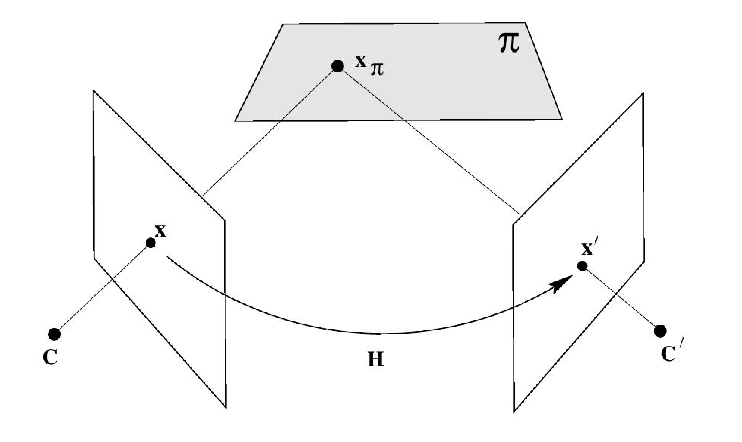
\includegraphics[scale=1.2]{homografia}
\caption{\textit{O mapeamento induzido por um plano no espaco 3D. O ponto $\x$ retroprojeta uma reta que intersecta o plano $\bpi$ no ponto $\X_{\bpi}$, então $\X_{\bpi}$ é projetado na outra imagem em $\x'$.}}
\label{fig.homografia}
\end{figure}
Na primeira câmera temos a projeção

\begin{equation*}
\x=P\,\X=[I|{\bf 0}]\,\X,
\end{equation*}
e qualquer ponto 3D do tipo $\X=(\x^\top,\rho)^\top$ vai satisfazer a projeção acima. De fato

\begin{equation*}
P\,\X=
[I|{\bf 0}]\,(\x^\top,\rho)^\top=
\begin{bmatrix}
1&0&0&0\\
0&1&0&0\\
0&0&1&0
\end{bmatrix}
\begin{pmatrix}
x_1\\
x_2\\
x_3\\
\rho
\end{pmatrix}
=\x,
\end{equation*}
e assim qualquer ponto na reta retroprojetada por $\x$ pode ser parametrizado por $\rho$. Como $\X\in\bpi$, $\bpi^\top\X=0$ e  
$\rho$ fica determinado

\begin{equation*}
\begin{array}{rcl}
\bpi^\top\,\X&=&0\\
({\bf v}^\top,1)\,(\x^\top,\rho)^\top&=&0\\
{\bf v}^\top\x+\rho&=&0\\
\rho&=&-{\bf v}^\top\,\x,
\end{array}
\end{equation*}
e dessa forma o ponto $\X=(\x^\top,-{\bf v}^\top\x)^\top$.
Projetando o ponto 3D na segunda imagem temos
\begin{equation*}
\begin{array}{rcl}
\x'&=&P'\X\\
&=&[R|{\bf t}]\,(\x^\top,-{\bf v}^\top\x)^\top\\
&=&R\,\x-{\bf t}\,{\bf v}^\top\x\\
&=&(R-{\bf t}\,{\bf v}^\top)\,\x.
\end{array}
\end{equation*}
Portanto

\begin{equation*}
\x'=H\,\x,\qquad\text{onde}\qquad H=R-{\bf t}\,{\bf v}^\top.
\end{equation*}


\subsubsection{A matriz fundamental $F$}\label{sec.matriz-F}

A \textit{matriz fundamental} reúne todas as informações da geometria epipolar, é a representação algébrica dessa geometria espacial com duas câmeras e, por isso, também é conhecida como \textit{tensor bifocal}. 

Geometricamente, a matriz fundamental pode ser obtida através do mapeamento de $\x$ na primeira imagem a um ponto $\x'$ na segunda imagem utilizando um plano $\bpi$ qualquer no espaço. Após esse mapeamento, identificamos a reta epipolar definida pelos pontos $\x'$ e $\e'$. Assim, considere um plano $\bpi$ que não passe pelos centros das câmeras, pois desse jeito uma reta retroprojetada por $\x$ deve interceptar o plano $\bpi$ em algum ponto $\X$. Usando a transferência através do plano $\bpi$, o ponto $\X$ deve ser projetado a um ponto $\x'$ na segunda imagem e, como $\X$ pertence à reta retroprojetada por $\x$, o ponto $\x'$ deverá pertencer à reta epipolar $\lightrgb'$, já que $\lightrgb'$ é a imagem na segunda câmera da reta retroprojetada por $\x$ conforme a figura \ref{fig.geo-epipolar}. Assim, pela subseção \ref{sec.homografia} existe uma homografia 2D $H$ em função de $\bpi$ onde cada ponto $\x_i$ é mapeado a um ponto $\x_i'$, 

\begin{equation}\label{eq.homo-plano}
\x'_i= H_{\bpi} \,\x_i.
\end{equation}
Tais pontos são ditos projetivamente equivalentes, já que são projetivamente equivalentes a um mesmo ponto $\X_i$ no plano $\bpi$. Obtido o ponto $\x'$, a reta epipolar passando por $\x'$ e $\e'$ pode ser calculada fazendo 

\begin{equation}\label{eq.reta-epi-pro-vet}
\begin{array}{rcl}
\lightrgb'&=&\e'\times\x'\\
&=&[\e']_\times\x'.
\end{array}
\end{equation}
Substituindo \ref{eq.homo-plano} em \ref{eq.reta-epi-pro-vet} temos

\begin{equation*}
\begin{array}{rcl}
\lightrgb'&=&[\e']_\times\x'\\
&=&[\e']_\times H_{\bpi} \,\x\\
&=&F\,\x,
\end{array}
\end{equation*} 
onde definimos $F=[\e']_\times H_{\bpi}$ é a matriz fundamental. Como $[\e']_\times$ é uma matriz anti-simétrica $3\times3$ obtida de um vetor, então  $[\e']_\times$ tem posto $2$ e como $H_{\bpi}$ obtida de um plano tem posto $3$, temos que a matriz fundamental tem posto $2$. $F$ é o mapeamento de um plano projetivo a um feixe de retas epipolares.


Algebricamente, a matriz fundamental pode ser determinada a partir das matrizes das duas câmeras $P$ e $P'$. Vamos primeiramente definir a equação que representa a reta retroprojetada por $\x$. Dado um ponto $\x$ na imagem, precisamos determinar o conjunto de pontos no espaço 3D que são mapeados nesse ponto $\x$, e este raio de luz (modelado por uma reta) será definido pela junção de dois de seus pontos. E conhecemos dois pontos pertencentes a esta reta, $\C$ é o centro da câmera tal que $P\,\C=0$, e o ponto $P^+\x$ onde $P^+$ é a pseudo-inversa de $P$ definida na subseção \ref{sec.Apen-A}. O ponto $P^+\x$ pertence à reta retroprojetada por $\x$ pois aplicando-lhe a projeção efetuada pela câmera temos o próprio ponto $\x$ como retorno:

\begin{equation*}
P^+\x \rightarrow P\,P^+\x=I\,\x=\x.
\end{equation*}
Portanto, podemos formar a reta pela junção dos pontos $\C$ e $P^+\x$, parametrizada por $\lambda$

\begin{equation*}
\X(\lambda)=P^+\x+\lambda\,\C.
\end{equation*}
Computando a imagem desses dois pontos na segunda câmera temos

\begin{equation*}
\begin{array}{c}
P^+\x \rightarrow P'P^+\x\\
\C \rightarrow P'\C,
\end{array}
\end{equation*}
onde $P'\,\C$ é o epipolo na segunda imagem, e por isso, a reta epipolar pode ser definida em termos do produto vetorial desses dois pontos

\begin{equation}\label{eq.reta-epipolar-funcao-cameras}
\lightrgb'=P'\C \times P'P^+\x.
\end{equation}
Mas como $P'\C=\e'$, podemos substitui-lo na equação anterior

\begin{equation*}
\begin{array}{rcl}
\lightrgb'&=&P'\C \times P'P^+\x\\
&=&[\e']_\times P'P^+\x\\
&=&F\,\x,
\end{array}
\end{equation*}
definindo $F=[\e']_\times P'P^+$. Essa relação para $F$ é a mesma fórmula derivada anteriormente, com a homografia planar calculada em termos das duas câmeras, $H_{\bpi}=P'P^+$.

Em problemas de reconstrução 3D podemos considerar a posição da primeira câmera como a origem do sistema de coordenadas do mundo, assim a matriz $P$, sua pseudo-inversa e a matriz da segunda câmera são, respectivamente 

\begin{equation*}
P=K\,[I|{\bf 0}],\qquad
P^+=
\begin{bmatrix}
K^{-1}\\
{\bf 0}^\top
\end{bmatrix}\qquad\text{e}\qquad
P'=K'[R|{\bf t}].
\end{equation*}
Substituindo na equação \ref{eq.reta-epipolar-funcao-cameras} temos

\begin{equation*}
\begin{array}{rcl}
\lightrgb'&=&P'\C \times P'P^+\x\\
&=&K'[R|{\bf t}]
\begin{pmatrix}
0\\
0\\
0\\
1
\end{pmatrix}
\times K'[R|{\bf t}]
\begin{bmatrix}
K^{-1}\\
{\bf 0}^\top
\end{bmatrix}\x\\
&=&
[K'{\bf t}]_\times K'\,R\,K^{-1}\x,
\end{array}
\end{equation*}
onde teremos uma nova definição para a matriz fundamental 
\begin{equation}\label{eq.definicao-F}
F=[K'{\bf t}]_\times K'\,R\,K^{-1}.
\end{equation}
Essa definição para $F$ é importante para falarmos sobre a matriz {\it essencial}.

\subsubsection{Propriedades da matriz fundamental}\label{sec.propriedades-F}
A partir da função $\x\rightarrow\lightrgb'$ dada pela relação $\lightrgb'=F\,\x$, podemos derivar a propriedade mais básica da matriz fundamental.
Observe que se $\x'\in\lightrgb'\Rightarrow\x'^\top\lightrgb'=0$, e temos
\begin{equation*}
\begin{array}{rcl}
\lightrgb'&=&F\,\x\\
\x'^\top\lightrgb'&=&\x'^\top F\,\x\\
0&=&\x'^\top F\,\x.
\end{array}
\end{equation*}
A relação acima é denominda {\it condição de correspondência}, pois pontos que a satisfazem devem ser  coplanares e tal relação se mostra uma ferramenta para a determinação da matriz fundamental a partir dos pontos correspondentes $\x\leftrightarrow\x'$. Observe que essa forma de determinar $F$ não requer o conhecimento das câmeras $P$ e $P'$. 

Se $F$ é a matriz para as câmeras $(P,P')$ então $F^\top$ é a matriz para $(P',P)$, pois basta aplicar a transposição em 
\begin{equation*}
\begin{array}{rcl}
\x'^\top F\,\x&=&0\\
\x^\top F^\top\x'&=&0,\quad\text{onde}\quad F^\top\x'=\lightrgb.
\end{array}
\end{equation*}

Os epipolos $\e$ e $\e'$ são os espaços nulos à direita e à esquerda de $F$, respectivamente. Vimos que $\e'\in\lightrgb'\Rightarrow\e'^\top\lightrgb'=0$, e $\lightrgb'=F\,\x$ para todo ponto $\x\in\lightrgb$ (exceto $\e$), daí
\begin{equation*}
\begin{array}{rcl}
\lightrgb'&=&F\,\x\\
\e'^\top\lightrgb'&=&\e'^\top F\,\x\\
0&=&\e'^\top F\,\x,\quad\text{para todo}\,\,\x\\
{\bf 0}^\top&=&\e'^\top F.
\end{array}
\end{equation*} 
A dedução é análoga para $F\,\e={\bf 0}$.

\subsubsection{Configuração canônica das câmeras}\label{sec.cameras-canonicas}
A relação $\lightrgb'=F\,\x$ é uma relação projetiva, já que envolve apenas relacionamentos projetivos entre os objetos geométricos, como interseção de retas e planos, e no desenvolvimento algébrico envolve apenas a projeção realizada pela câmera entre pontos no mundo e pontos na imagem. Com isso, a relação depende apenas das coordenadas projetivas da imagem, ou seja, é projetivamente invariante. Assim, dadas transformações projetivas das imagens $\hat{\x}=H\,\x$ e $\hat{\x}'=H'\x'$ podemos deduzir a correspondente relação $\hat{\lightrgb}'=\hat{F}\hat{\x}$ com $\hat{F}=H'^{-\top}F\,H^{-1}$. Analogamente, $F$ depende somente das propriedades projetivas das câmeras $P$ e $P'$, já que as imagens são geradas pela ação dessas duas câmeras. As câmeras dependem tanto do sistema de coordenadas das imagens como do sistema de coordenadas do mundo, mas a matriz fundamental é inalterável por uma transformação projetiva do espaço 3D. 

Observe que se $H_{4\times4}$ é uma transformação projetiva do espaço 3D, então as relações de projeção podem ser escritas como
\begin{equation*}
\begin{array}{rcl}
\x&=&P\,\X\\
\x&=&P\,H\,H^{-1}\X
\end{array}\qquad\text{e}\qquad
\begin{array}{rcl}
\x'&=&P'\X\\
\x'&=&P'H\,H^{-1}\X
\end{array}.
\end{equation*} 
Se $\x\leftrightarrow\x'$ é uma correspondência para o par de câmeras $(P,P')$ em relação ao ponto $\X$, então essas imagens também são correspondentes para o par de câmeras $(P\,H,P'H)$ em relação ao ponto $H^{-1}\X$. Como a matriz fundamental depende apenas das coordenadas das imagens (\ref{sec.propriedades-F}), temos que a matriz fundamental para $(P,P')$ será a mesma para $(P\,H,P'H)$. Ou seja, um par de câmeras unicamente define uma matriz fundamental, mas uma matriz fundamental é consistente com vários pares de câmeras.

Já que temos vários pares de câmeras consistentes com a mesma matriz fundamental, podemos escolher um par de câmeras, através de uma transformação projetiva, de forma que algumas futuras abordagens e deduções sejam facilitadas sem prejuízo das características projetivas. Dadas câmeras calibradas $\hat{P}$ e $\hat{P'}$ podemos acrescentar uma linha em $\hat{P}$ de forma que se torne uma matriz $4\times4$ invertível denotada por $\hat{P}^*$. Aplicando a inversa de $\hat{P}^*$ em $\hat{P}$ e $\hat{P}'$ temos que
\begin{equation*}
\begin{array}{rcl}
P&=&\hat{P}\,\hat{P}^{*-1}\\
P&=&[I|{\bf 0}]
\end{array}\qquad\text{e}\qquad
\begin{array}{rcl}
P'&=&\hat{P}'\,\hat{P}^{*-1}\\
P'&=&[M|{\bf m}].
\end{array}
\end{equation*}
As câmeras $P$ e $P'$ definidas acima estão em sua forma {\it canônica}. Observe, pela dedução da equação \ref{eq.definicao-F}, que a matriz fundamental para câmeras canônicas é simplesmente 
\begin{equation*}
F=[{\bf m}]_\times M.
\end{equation*}


\subsubsection*{Extraindo as câmeras canônicas a partir de $F$}
Nesta seção será apresentada uma das formas de se obter as matrizes das câmeras para um sistema com duas visões. Como vimos na subseção \ref{sec.cameras-canonicas}, é possível aplicar uma transformação projetiva de forma a se obter o par de câmeras canônicas para um sistema bifocal, e assim facilitar o algebrismo e a computação sem prejuízo das características projetivas do sistema. Desta forma, dada a matriz $F$ computada através da codição de correspondência, vamos mostrar como extrair o par de câmeras em sua forma canônica.

Primeiramente, observe pelo apêndice \ref{sec.Apen-A} o caso $3\times3$ em que uma matriz $M$ é anti-simétrica se satisfaz a condição ${\bf v}^\top M\,{\bf v}=0$. Considerando a matriz $P'^\top F\,P$, a mesma será anti-simétrica se $\X^\top P'^\top F\,P\,\X=0$. Mas $\x=P\,\X$ e $\x'^\top=\X^\top P'^\top$, e substituindo temos que $\x'^\top F\,\x=0$. Pela subseção \ref{sec.propriedades-F}, essa condição de correspondência mostra que $F$ é a matriz fundamental consistente com o par de câmeras $(P,P')$ já que $P'^\top F\,P$ seja anti-simétrica.

Agora, tomando a configuração canônica $P=[I|{\bf 0}]$ e $P'=[SF\,|\e']$, onde $S$ é uma matriz anti-simétrica e $\e'$ é o epipolo que satisfaz $\e'^\top F={\bf 0}^\top$ (subseção \ref{sec.propriedades-F}), temos que $P'^\top F\,P$ é anti-simétrica, pois
\begin{equation*}
P'^\top F\,P=[SF\,|\e']^\top F\,[I|{\bf 0}]=
\begin{bmatrix}
F^\top S^\top F&{\bf 0}\\
\e'^\top F&0
\end{bmatrix}=
\begin{bmatrix}
F^\top S^\top F&{\bf 0}\\
{\bf 0}^\top&0
\end{bmatrix}.
\end{equation*}
Assim, dada $F$ temos que um par de câmeras consistente é simplesmente $P=[I|{\bf 0}]$ e $P'=[SF\,|\e']$. Repare que a escolha da matriz $S$ é arbitrária mas com a exigência de que a matriz $P'$ deve ter posto 3 para ser uma câmera válida. Isso não é problema pois segundo \citep{luong} uma boa escolha é $S=[\e']_\times$ pois $\e'$ não pertence ao espaço gerado pelas colunas de $[\e']_\times F$. Finalmente, o par de câmeras canônicas pode ser obtido tomando 
\begin{equation}\label{eq.cameras-dada-F}
P=[I|{\bf 0}]\qquad\text{e}\qquad P'=[[\e']_\times F\,|\e'].
\end{equation}

\subsubsection{Ambiguidade projetiva das câmeras, dada $F$}\label{sec.ambi-cameras-dada-F}

De uma matriz fundamental podemos extrair diferentes pares de câmeras consistentes com a mesma geometria epipolar, em contraste com o fato de, dado um par de câmeras, a matriz fundamental ser única. Esses pares de câmeras extraídas de $F$ diferem apenas por uma transformação projetiva.

Inicialmente, podemos aplicar uma transformação projetiva e trabalhar com a forma canônica das câmeras $P=\tilde{P}=[I|{\bf 0}]$, $P'=[A|{\bf a}]$ e $\tilde{P}'=[\tilde{A}|\tilde{{\bf a}}]$. Evocando o resultado em \ref{sec.cameras-canonicas} sabemos que a matriz fundamental pode ser obtida fazendo 
$F=[{\bf a}]_{\times} A=[\tilde{{\bf a}}]_{\times} \tilde{A}$. Como $[{\bf a}]_{\times}$ e $[\tilde{{\bf a}}]_{\times}$ são anti-simétricas temos que
\begin{equation*}
{\bf a}^\top F={\bf a}^\top [{\bf a}]_{\times} A={\bf 0}^\top\quad\text{e}\quad\tilde{{\bf a}}^\top F=\tilde{{\bf a}}^\top [\tilde{{\bf a}}]_{\times} \tilde{A}={\bf 0}^\top,
\end{equation*}
e como $F$ tem posto 2 e não pode ser invertida, temos que ${\bf a}^\top$ e ${\tilde{{\bf a}}^\top}$ são iguais a menos de escala, portanto
\begin{equation}\label{eq.dedu-ambiguidade-P-1}
{\tilde{{\bf a}}^\top}=k\,{\bf a}^\top.
\end{equation}
Considerando $[{\bf a}]_{\times} A=[\tilde{{\bf a}}]_{\times} \tilde{A}$ e substituindo \ref{eq.dedu-ambiguidade-P-1} temos
\begin{equation*}
\begin{array}{rcl}
[{\bf a}]_{\times} A&=&k\,[{\bf a}]_{\times} \tilde{A}\\
0_{3\times3}&=&k\,[{\bf a}]_{\times} \tilde{A}-[{\bf a}]_{\times} A\\
0_{3\times3}&=&[{\bf a}]_{\times}(k\,\tilde{A}-A).
\end{array}
\end{equation*}
Já que ${\bf a}$ é um vetor nulo à direita de $[{\bf a}]_{\times}$ podemos tomar, para um vetor ${\bf v}$ qualquer,
\begin{equation}\label{eq.dedu-ambiguidade-P-2}
k\,\tilde{A}-A={\bf a}{\bf v}^\top\quad\text{e daí}\quad \tilde{A}=\frac{A+{\bf a}{\bf v}^\top}{k}. 
\end{equation}
Substituindo as equações \ref{eq.dedu-ambiguidade-P-1} e \ref{eq.dedu-ambiguidade-P-2} na câmera $\tilde{P}'$ temos que 
\begin{equation}\label{eq.camera-geral}
P'=[A|{\bf a}]\quad\text{e}\quad \tilde{P}'=[k^{-1}(A+{\bf a}{\bf v}^\top)|k\,{\bf a}],
\end{equation}
e vamos usar a homografia
\begin{equation*}
H=
\begin{bmatrix}
k^{-1}I&{\bf 0}\\
k^{-1}{\bf v}^\top&k
\end{bmatrix}
\end{equation*}
para mostrar que as câmeras estão projetivamente relacionadas.
\begin{equation*}
PH=[I|{\bf 0}]
\begin{bmatrix}
k^{-1}I&{\bf 0}\\
k^{-1}{\bf v}^\top&k
\end{bmatrix}
=
k^{-1}[I|{\bf 0}]=k^{-1}\tilde{P},\quad\text{e}
\end{equation*}
\begin{equation*}
P'H=[A|{\bf a}]
\begin{bmatrix}
k^{-1}I&{\bf 0}\\
k^{-1}{\bf v}^\top&k
\end{bmatrix}
=
[k^{-1}(A+{\bf a}{\bf v}^\top)|k\,{\bf a}]
=[\tilde{A}|\tilde{{\bf a}}]=\tilde{P}'.
\end{equation*}
Juntando a extração das câmeras dada em \ref{eq.cameras-dada-F} com a equação geral para câmeras dada em \ref{eq.camera-geral} temos a fórmula geral para câmeras canônicas dada a matriz fundamental
\begin{equation*}
P=[I|{\bf 0}]\quad\text{e}\quad P'=[[\e']_\times F+\e'{\bf v}^\top |\lambda\,\e'],
\end{equation*} 
para um vetor ${\bf v}$ qualquer  e um escalar $\lambda\neq0$.

\subsubsection*{A matriz essencial $E$}
Historicamente, a matriz essencial foi introduzida antes da matriz fundamental e pode ser pensada como um caso particular da matriz fundamental \citep{Longuet}, onde os efeitos da matriz de calibração $K$ foram removidos da câmera $P$. Considere uma câmera $P=K\,[R|{\bf t}]$ onde conhecemos sua matriz de calibração. Podemos inverter a matriz $K$ e aplicá-la na câmera de modo que a projeção se torne $P=[R|{\bf t}]$, chamada {\it câmera normalizada}. Aplicando essa projeção a um ponto no espaço 3D $\X$ temos 
\begin{equation*}
\hat{\x}=P\,\X=[R|{\bf t}]\,\X
\end{equation*}
onde o ponto $\hat{\x}$ é dito estar em {\it coordenadas  normalizadas}. Um par de câmeras normalizadas 
\begin{equation*}
P=[I|{\bf 0}]\qquad\text{e}\qquad P'=[R|{\bf t}]
\end{equation*}
tem a matriz {\it essencial} como matriz correspondente que reúne todas as características relativas à geometria epipolar para essas duas câmeras. Usando a derivação da matriz fundamental na equação \ref{eq.definicao-F}, podemos definir a matriz essencial
\begin{equation*}
E=[{\bf t}]_\times R.
\end{equation*}

\newpage
\section{Reconstrução de uma câmera $P$: desenvolvimento da abordagem de \citep{bib:kuang}.}\label{sec.astrom}
Uma câmera pode ser fatorada em $P=K[R|{\bf t}]$, e o artigo \citep{bib:kuang} trata da determinação dos parâmetros externos $R$ e ${\bf t}$, considerando que são conhecidos quase todos os parâmetros internos da matriz $K$, menos a distância focal $f$. Assim, o artigo busca determinar sete parâmetros no total, três na matriz de rotação $R$, três no vetor de translação ${\bf t}$ e um na matriz de calibração. Alguns trabalhos anteriores já resolveram problemas de determinação desses sete parâmetros mas todos eles usaram somente correspondência entre pontos 3D e pontos 2D, $\X\leftrightarrow\x$, e as principais contribuições de \citep{bib:kuang} são o uso de correspondências entre outras entidades geométricas como retas e pontos-tangentes, e a apresentação de um procedimento para resolução de sistemas de equações polinomiais utilizando as Bases de Gr\"obner e a Matriz de Ação. 

Como já vimos, os parâmetros externos $R$ e ${\bf t}$ tem a finalidade de trazer um ponto 3D escrito no sistema de coordenadas do mundo para o sistema de coordenadas da câmera, e na figura \ref{fig.camera-astrom} podemos observar a ação de $[R|{\bf t}]$ bem como a correspondência entre entidades geométricas.

\begin{figure}[!htb]
\centering
\includegraphics[scale=.8]{camera-astrom}
\caption{{\it A matriz $[R|{\bf t}]$ transforma as estruturas 3D em coordenadas do mundo para as coordenadas da câmera, deixando-as em coordenadas normalizadas. Depois que as estruturas estão em coordenadas normalizadas, a matriz $K$ faz a projeção no plano da imagem final, aplicando características como tamanho dos pixels, distância focal, ponto principal e inclinação entre eixos.}}
\label{fig.camera-astrom}
\end{figure}

\subsection{Formulação do problema}

O artigo utiliza o modelo {\it pinhole} de câmera para aplicar a projeção de um ponto $\X$ em 3D em sua imagem $\x$ em 2D dada pela equação de projeção
\begin{equation}\label{eq.projecao}
\lambda\,\x=P\,\X,
\end{equation}
onde a matriz $P_{3\times4}$ pode ser fatorada conforme descrito acima, e $\lambda$ é um fator de escala descrito na subseção \ref{sec.ponto}. 

Para obter estabilidade numérica e uma configuração prática da câmera, geralmente se assume que o plano da imagem tem o ponto principal centrado na origem, pixels quadrados e eixos perpendiculares ({\it skew} zero). Como a única incógnita na matriz de calibração é a distância focal, a mesma pode ser descrita como
\begin{equation}\label{eq.astrom-K}
K=
\begin{bmatrix}
1&0&0\\
0&1&0\\
0&0&w
\end{bmatrix},
\end{equation}
onde $w=\frac{1}{f}$.

\subsubsection*{Quantidade de equações}

Cada objeto geométrico nos fornece uma quantidade de equações para determinarmos os parâmetros de $P$, e vamos analisar de que forma esses objetos providenciam as equações. Na figura \ref{fig.astrom-objetos-geo} podemos visualizar um exemplo de cada uma das entidades geométricas.

\begin{figure}[!htb]
\centering
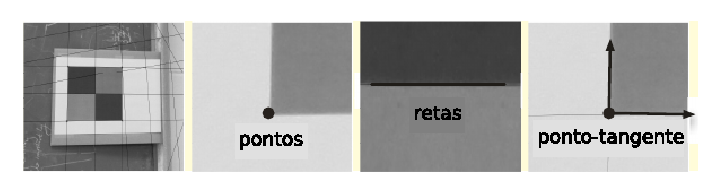
\includegraphics[scale=1]{astrom-objetos-geo}
\caption{{\it Objetos utilizados para gerar equações na determinação dos parâmetros de $P$.}}
\label{fig.astrom-objetos-geo}
\end{figure}

\subsubsection*{Equações obtidas usando pontos}

Dado um ponto 3D $\X$ e sua respectiva imagem em 2D $\x=(x,y,1)^\top$, a equação de projeção $\lambda\,\x=P\,\X$ nos fornece três equações. Mas, pela subseção \ref{sec.ponto}, um ponto 2D tem apenas dois graus de liberdade apesar de suas três componentes, então dessas três equações apenas duas são linearmente independentes. Para eliminarmos o fator de escala $\lambda$ aplicamos o produto vetorial em ambos os lados da equação de projeção:
\begin{equation}\label{eq.astrom-pontos}
\begin{array}{rcl}
\lambda\,\x&=&P\,\X\\
\lambda\,[\x]_\times\x&=&[\x]_\times P\,\X\\
{\bf 0}&=&[\x]_\times P\,\X.
\end{array}
\end{equation}

\subsubsection*{Equações obtidas usando retas} 

Uma reta 3D ${\bf L}$ pode ser representada usando um ponto $\X$ e uma direção ${\bf D}$, na forma ${\bf L}=\X+k\,{\bf D}$. Dadas a reta ${\bf L}$ e sua imagem $\lightrgb$ obtemos duas equações usando os dois pontos $\X$ e ${\bf D}$. Um ponto $\x$ pertence a uma reta $\lightrgb$ se $\lightrgb^\top\x=0$, e substituindo essa relação na equação de projeção \ref{eq.projecao} temos
\begin{equation}\label{eq.astrom-retas}
\begin{array}{rcll}
\lightrgb^\top P\,\X&=&0&\text{se}\,\,\,k=0\\
\lightrgb^\top P(\X+k\,{\bf D})&=&0&\text{se}\,\,\,k\neq0.
\end{array}
\end{equation}  

\subsubsection*{Equações obtidas usando pontos-tangentes}

É possível obter mais três equações se conhecemos o ponto $\X$, uma direção ${\bf D}$ através $\X$ bem como suas respectivas imagens $\x$ e ${\bf d}$. Com a correspondência $\X\leftrightarrow\x$ podemos usar a relação \ref{eq.astrom-pontos} e conseguir duas equações. Para a terceira equação, usamos a reta definida pelos pontos na imagem, $\lightrgb=\x\times{\bf d}$, juntamente com as relações em \ref{eq.astrom-retas}, pois tomando a diferença entre as relações em \ref{eq.astrom-retas} e usando a reta $\lightrgb$ temos
\begin{equation}\label{eq.astrom-direcao}
\lightrgb^\top P\,{\bf D}=0.
\end{equation}  

Note que essas três equações são obtidas usando um ponto-tangente com uma direção apenas. Se usarmos ponto-tangente com mais direções, conseguimos uma equação a mais para cada direção, pois para cada ${\bf D}_i$ das $n$ direções, teremos $\lightrgb_i=\x\times{\bf d}_i$ e podemos formular as equações
\begin{equation}
[\x]_\times P\,\X={\bf 0}\quad\text{e}\quad\lightrgb_i^\top P\,{\bf D}_i=0\quad\text{para}\,\,i=1,...,n.
\end{equation}

Na tabela abaixo podemos verificar um resumo da quantidade de equações conseguidas para correspondências entre cada objeto geométrico.
\begin{center}
\begin{tabular}{|c|c|c|c|}
\hline 
{\bf ponto} & {\bf reta} & {\bf ponto com 1 tangente} & {\bf ponto com 2 tangentes} \\ 
\hline 
2 & 2 & 3 & 4 \\ 
\hline 
\end{tabular} 
\end{center}

\subsubsection*{Casos úteis}

Com as quantidades de equações fornecidas por cada correspondência podemos formar várias combinações entre pontos, retas e ponto-tangentes para obtermos as sete equações necessárias para calcular os sete graus de liberdade de $P$. Vamos ver dois exemplos de problema mínimo.
\begin{itemize}
\item {\bf Dois pontos e um ponto-tangente (P2T1)}: com essa combinação temos três pontos e uma direção passando por um dos pontos, então podemos formar seis equações usando a relação \ref{eq.astrom-pontos} e mais uma equação usando a relação \ref{eq.astrom-direcao}. 

\item {\bf Um ponto-tangente com uma direção mais um ponto-tangente com duas direções (T1T2)}: temos uma reta passando por um dos pontos e duas retas passando pelo outro ponto, então podemos formar quatro equações usando \ref{eq.astrom-pontos} e mais três equações usando \ref{eq.astrom-direcao}.
\end{itemize} 

Podemos formar outros problemas mínimos conforme os apresentados aqui e vamos mostrar agora um caso supra-restringido, onde temos mais equações do que incógnitas a determinar.
\begin{itemize}
\item {\bf Quatro retas (P4L)}: Dadas quatro correspondências entre retas temos oito equações usando as relações \ref{eq.astrom-retas}. Como precisamos de sete equações podemos usar uma delas para verificar a solução dada pelas demais.
\end{itemize}

\subsubsection*{Parametrização de $P$}

Uma das ideias teóricas mais importantes do método e que a matriz de rotação da câmera é parametrizada com quaternions, pois desse modo produz sistemas de equações polinomiais relativamente fáceis de serem resolvidos. Utilizando quaternions, a matriz de rotação é dada por
\begin{equation*}
R=
\begin{bmatrix}
a^2+b^2-c^2-d^2&2bc-2ad&2ac+2bd\\
2ad+2bc&a^2-b^2+c^2-d^2&2cd-2ab\\
2bd-2ac&2ab+2cd&a^2-b^2-c^2+d^2
\end{bmatrix}
\end{equation*}
Se tratando de uma representação em coordenadas homogêneas podemos usar uma das variáveis para fixar a escala, assim tomando $a=1$ reduzimos o número de variáveis e facilitamos a solução do sistema de equações polinomiais.

O vetor de translação é parametrizado normalmente como ${\bf t}=(t_x,t_y,t_z)^\top$ e a matriz $[R|{\bf t}]$ se torna
\begin{equation*}
[R|{\bf t}]=
\begin{bmatrix}
a^2+b^2-c^2-d^2&2bc-2ad&2ac+2bd&t_x\\
2ad+2bc&a^2-b^2+c^2-d^2&2cd-2ab&t_y\\
2bd-2ac&2ab+2cd&a^2-b^2-c^2+d^2&t_z
\end{bmatrix}
\end{equation*}
Para completar a matriz $P$ basta aplicar, à esquerda de $[R|{\bf t}]$ a matriz de calibração $K$ conforme \ref{eq.astrom-K}.
\begin{equation*}
\begin{array}{rcl}
P&=&K\,[R|{\bf t}]\\\\
&=&
\begin{bmatrix}
1&0&0\\
0&1&0\\
0&0&w
\end{bmatrix}
\begin{bmatrix}
a^2+b^2-c^2-d^2&2bc-2ad&2ac+2bd&t_x\\
2ad+2bc&a^2-b^2+c^2-d^2&2cd-2ab&t_y\\
2bd-2ac&2ab+2cd&a^2-b^2-c^2+d^2&t_z
\end{bmatrix}\\\\
&=&
\begin{bmatrix}
a^2+b^2-c^2-d^2&2bc-2ad&2ac+2bd&t_x\\
2ad+2bc&a^2-b^2+c^2-d^2&2cd-2ab&t_y\\
w\,(2bd-2ac)&w\,(2ab+2cd)&w\,(a^2-b^2-c^2+d^2)&w\,t_z
\end{bmatrix}
\end{array}
\end{equation*} 

Substituindo $t'_z=w\,t_z$, temos que determinar as sete variáveis $\{b,c,d,t_x,t_y,t'_z,w\}$. Mas observe que as variáveis $\{t_x,t_y,t'_z\}$ são todas lineares usando as relações \ref{eq.astrom-pontos}, \ref{eq.astrom-retas} e \ref{eq.astrom-direcao}, e portanto podem ser eliminadas do sistemas de equações restando apenas as quatro variáveis $\{b,c,d,w\}$. Depois de determinadas essas quatro variáveis, o vetor de translação pode ser recuperado por substituição. 

\subsection{Sistema de equações polinomiais}

Para resolver computacionalmente os sistemas de equações polinomiais decorrentes do emprego dos casos úteis na determinação de $P$, \citep{bib:kuang} utiliza metodos baseados em Geometria Algébrica. Primeiramente, utilizando a ferramenta {\it Macaulay2} \citep{macaulay2}, é verificada a existência de 20 soluções para o caso mínimo (P2T1). Para sistemas com pouca quantidade de variáveis, usar apenas o método das Bases de Gr\"obner pode ser rápido e numericamente estável, mas aqui é empregado o método exposto em \citep{byrod}, que consiste basicamente em extrair a Base Linear a partir das Bases de Gr\"obner e empregar a Matriz de Ação, da qual as soluções podem ser obtidas pela decomposição em autovalores. No apêndice \ref{sec.geo-algebrica} é fornecido um resumo sobre a teoria básica de Geometria Algébrica, bem como exemplos da utilização do método das Bases de Gr\"obner e da Matriz de Ação para resolver sistemas.




